% This is a template for Ph.D. dissertations in the UCI format.
% 
% All fonts, including those for sub- and superscripts, must be 10
% points or larger.  Recommended sizes are 14-point for chapter
% headings, 12-point for the main body of text and figure/table
% titles, and 10-point for footnotes, sub- and super-scripts, and text
% in figures and tables.
%
% Notes: Add short title to figures, sections, via square brackets,
% e.g. \section[short]{long}.
%
\documentclass[12pt,fleqn]{ucithesis}

% A few common packages
\usepackage{amsmath}
\usepackage{amsthm}
\usepackage{array}
\usepackage{graphicx}
\usepackage[round]{natbib}
\usepackage{relsize}
\usepackage[titletoc]{appendix}

% Some other useful packages
\usepackage{caption}
\usepackage{subcaption}  % \begin{subfigure}...\end{subfigure} within figure
\usepackage{multirow}
\usepackage{tabularx}

\usepackage{siunitx}
\usepackage{algorithm}
\usepackage{algpseudocode}
\usepackage{upgreek}
\usepackage{url}
\usepackage{amsfonts}

% Uncomment the following to attempt to enforce Type 1 or TrueType 
% fonts. ProQuest does not want the type 3 fonts used by default as
% of Dec. 2019 - see 
% https://support.proquest.com/articledetail?id=kA01W000000k9o2SAA . 
% If you are unable to embed fonts such as 'Zapf Dingbats' or 
% 'Symbol', try using raster images (.jpg or .png) instead of vector 
%images (.pdf or .eps).
% \usepackage[T1]{fontenc} 

% plainpages=false fixes the "duplicate ignored" error with page counters
% Set pdfborder to 0 0 0 to disable colored borders around PDF hyperlinks
\usepackage[plainpages=false,pdfborder={0 0 0}]{hyperref}

% Uncomment the following line to use the algorithm package,
% which provides an algorithm environment similar to figure and table
% ("\begin{algorithm}...\end{algorithm}"). A list of algorithms will
% automatically be added in the preliminary pages. Note that you
% probably want a package for the actual code to go with this (e.g.,
% algorithmic).
%\usepackage{algorithm}

% Uncomment the following line to enable Unicode support. This will allow you
% to enter non-ASCII characters (such as accented characters) directly without
% having to use LaTeX's awkward escape syntax (e.g., \'{e})
% NOTE: You may have to install the ucs.sty package for this to work. See:
% http://www.unruh.de/DniQ/latex/unicode/
%\usepackage[utf8x]{inputenc}

% Uncomment the following to avoid "widowing", where page breaks cause
% single lines of paragraphs to float onto the next page (this is not
% a UCI requirement but more of an aesthetic choice).
%\widowpenalty=10000
%\clubpenalty=10000


\def\bSig\mathbf{\Sigma}
\newcommand{\VS}{V\&S}
\newcommand{\tr}{\mbox{tr}}
\DeclareMathOperator{\E}{\mathbb{E}}
\DeclareMathOperator{\x}{\mathbf{x}}

% Modify or extend these at will.
\newtheorem{theorem}{\textsc{Theorem}}[chapter]
\newtheorem{definition}{\textsc{Definition}}[chapter]
\newtheorem{example}{\textsc{Example}}[chapter]

% Macros for title, author, abstract, etc.
\thesistitle{Title of the Thesis}

%"Dissertation" for PhD, "Thesis" for master's
\documenttitle{Dissertation}

\degreename{Doctor of Philosophy}

% Use the wording given in the official list of degrees awarded by UCI:
% http://www.rgs.uci.edu/grad/academic/degrees_offered.htm
\degreefield{Statistics}

% Your name as it appears on official UCI records.
\authorname{Your name}

% Use the full name of each committee member and full title 
% (e.g. Professor/Associate Professor).
\committeechair{Professor A}
\othercommitteemembers
{
  Assistant Professor B\\
  Associate Professor C
}

\degreeyear{2012}

\copyrightdeclaration
{
  {\copyright} {\Degreeyear} \Authorname
}

% If you have previously published parts of your manuscript, you must list the
% copyright holders; see Section 3.2 of the UCI Thesis and Dissertation Manual.
% Otherwise, this section may be omitted.
% \prepublishedcopyrightdeclaration
% {
% 	Chapter 4 {\copyright} 2003 Springer-Verlag \\
% 	Portion of Chapter 5 {\copyright} 1999 John Wiley \& Sons, Inc. \\
% 	All other materials {\copyright} {\Degreeyear} \Authorname
% }

% The dedication page is optional
% (comment out to exclude).
\dedications
{
  (Optional dedication page)
  
  To ...
}

\acknowledgments
{
  I would like to thank...
  
  (You must acknowledge grants and other funding assistance. 
  
  You may also acknowledge the contributions of professors and
  friends.
  
  You also need to acknowledge any publishers of your previous
  work who have given you permission to incorporate that work
  into your dissertation. See Section 3.2 of the UCI Thesis and
  Dissertation Manual.)
}


% Some custom commands for your list of publications and software.
\newcommand{\mypubentry}[3]{
  \begin{tabular*}{1\textwidth}{@{\extracolsep{\fill}}p{4.5in}r}
    \textbf{#1} & \textbf{#2} \\ 
    \multicolumn{2}{@{\extracolsep{\fill}}p{.95\textwidth}}{#3}\vspace{6pt} \\
  \end{tabular*}
}
\newcommand{\mysoftentry}[3]{
  \begin{tabular*}{1\textwidth}{@{\extracolsep{\fill}}lr}
    \textbf{#1} & \url{#2} \\
    \multicolumn{2}{@{\extracolsep{\fill}}p{.95\textwidth}}
    {\emph{#3}}\vspace{-6pt} \\
  \end{tabular*}
}

% Include, at minimum, a listing of your degrees and educational
% achievements with dates and the school where the degrees were
% earned. This should include the degree currently being
% attained. Other than that it's mostly up to you what to include here
% and how to format it, below is just an example.
%
% CV is required for PhD theses, but not Master's
% comment out to exclude
\curriculumvitae
{

\textbf{EDUCATION}
  
  \begin{tabular*}{1\textwidth}{@{\extracolsep{\fill}}lr}
    \textbf{Doctor of Philosophy in Computer Science} & \textbf{2012} \\
    \vspace{6pt}
    University name & \emph{City, State} \\
    \textbf{Bachelor of Science in Computational Sciences} & \textbf{2007} \\
    \vspace{6pt}
    Another university name & \emph{City, State} \\
  \end{tabular*}

\vspace{12pt}
\textbf{RESEARCH EXPERIENCE}

  \begin{tabular*}{1\textwidth}{@{\extracolsep{\fill}}lr}
    \textbf{Graduate Research Assistant} & \textbf{2007--2012} \\
    \vspace{6pt}
    University of California, Irvine & \emph{Irvine, California} \\
  \end{tabular*}

\vspace{12pt}
\textbf{TEACHING EXPERIENCE}

  \begin{tabular*}{1\textwidth}{@{\extracolsep{\fill}}lr}
    \textbf{Teaching Assistant} & \textbf{2009--2010} \\
    \vspace{6pt}
    University name & \emph{City, State} \\
  \end{tabular*}

\pagebreak

\textbf{REFEREED JOURNAL PUBLICATIONS}

  \mypubentry{Ground-breaking article}{2012}{Journal name}

\vspace{12pt}
\textbf{REFEREED CONFERENCE PUBLICATIONS}

  \mypubentry{Awesome paper}{Jun 2011}{Conference name}
  \mypubentry{Another awesome paper}{Aug 2012}{Conference name}

\vspace{12pt}
\textbf{SOFTWARE}

  \mysoftentry{Magical tool}{http://your.url.here/}
  {C++ algorithm that solves TSP in polynomial time.}

}

% The abstract was previously limited to a maximum of 350 words, 
% but the UCI manual at https://etd.lib.uci.edu/electronic/td2e#2.2.1.
% currently does not indicate that there is any word limit for the abstract
\thesisabstract
{
  The abstract of your contribution goes here.
}


%%% Local Variables: ***
%%% mode: latex ***
%%% TeX-master: "thesis.tex" ***
%%% End: ***


% Add PDF document info fields
\hypersetup{
	pdftitle={\Thesistitle},
	pdfauthor={\Authorname},
	pdfsubject={\Degreefield},
}

% Uncomment the following to have numbered subsubsections (by default
% numbering goes only to subsections).
%\setcounter{secnumdepth}{4}


% Set this to only select a subset of the includes directives below.
% Very handy to speed up compilation if you're working on a certain
% part of your thesis. It conserves page numbers, references, etc.
% even for non-included files.
%\includeonly{chapter1}

\begin{document}

% Preliminary pages are always loaded (TOC, CV, etc.)
\preliminarypages

% Include the different components of your thesis, in separate files.
% Using \include allows you to set \includeonly above.
\chapter{Introduction}

In epidemiology studies, geospatial disparities of certain disease risks are of common interest since the potential unequal risks could be a result of location-related risk factors. These factors could be environmental, demographic, socioeconomic among others. Thus, spatial epidemiologists frequently aim to estimate a risk pattern over an area under study, which is frequently a residential geospatial area. 

This is an example using the \LaTeX{} template for UCI theses and
dissertation documents \cite{uci-thesis-latex}. Figure
\ref{fig:sourcecode} is just for illustration purposes, as is Table
\ref{tab:coordinates}.

\begin{figure}
\begin{verbatim}
#include <iostream>
int main(int argc, char** argv) {
  std::cout << "Hello World." << std::endl;
  return 0;
}
\end{verbatim}
  \caption{Example source code.}
  \label{fig:sourcecode}
\end{figure}

\section{Background}

Lorem ipsum dolor sit amet, consectetur adipisicing elit, sed do
eiusmod tempor incididunt ut labore et dolore magna aliqua. Ut enim ad
minim veniam, quis nostrud exercitation ullamco laboris nisi ut
aliquip ex ea commodo consequat. Duis aute irure dolor in
reprehenderit in voluptate velit esse cillum dolore eu fugiat nulla
pariatur. Excepteur sint occaecat cupidatat non proident, sunt in
culpa qui officia deserunt mollit anim id est laborum.

\begin{table}
  \centering
  \begin{tabular}{|rr|r|}
    \hline
    $x$ & $y$ & $z$ \\
    \hline
    14 & 12 & -2 \\
    0 & 33 & -25 \\
    -3 & 11 & 22 \\
    4 & 4 & 6 \\
    \hline
  \end{tabular}
  \caption{Example coordinates.}
  \label{tab:coordinates}
\end{table}

Lorem ipsum dolor sit amet, consectetur adipisicing elit, sed do
eiusmod tempor incididunt ut labore et dolore magna aliqua. Ut enim ad
minim veniam, quis nostrud exercitation ullamco laboris nisi ut
aliquip ex ea commodo consequat. Duis aute irure dolor in
reprehenderit in voluptate velit esse cillum dolore eu fugiat nulla
pariatur. Excepteur sint occaecat cupidatat non proident, sunt in
culpa qui officia deserunt mollit anim id est laborum.


%%% Local Variables: ***
%%% mode: latex ***
%%% TeX-master: "thesis.tex" ***
%%% End: ***

%\chapter{Statistical background}

Conditional AIC

\begin{equation}
\textbf{cAIC}=-2log(L(y|\hat{\beta}(y),\hat{b}(y))L(\hat{b}(y)|\hat{\alpha}(y)))+2p
%\textbf{cAIC}=-2\L(y|\hat{\beta}(y),\hat{b}(y))L(\hat{b}|\hat{\alpha})+2p
\end{equation}


In epidemiology studies, geospatial disparities of certain disease risks are of common interest since the potential unequal risks could be a result of location-related risk factors. These factors could be environmental, demographic, socioeconomic among others. Thus, spatial epidemiologists frequently aim to estimate a risk pattern over an area under study, which is frequently a residential geospatial area. 

This is an example using the \LaTeX{} template for UCI theses and
dissertation documents \cite{uci-thesis-latex}. Figure
\ref{fig:sourcecode} is just for illustration purposes, as is Table
\ref{tab:coordinates}.

\begin{figure}
\begin{verbatim}
#include <iostream>
int main(int argc, char** argv) {
  std::cout << "Hello World." << std::endl;
  return 0;
}
\end{verbatim}
  \caption{Example source code.}
  \label{fig:sourcecode}
\end{figure}

\section{Background}

Lorem ipsum dolor sit amet, consectetur adipisicing elit, sed do
eiusmod tempor incididunt ut labore et dolore magna aliqua. Ut enim ad
minim veniam, quis nostrud exercitation ullamco laboris nisi ut
aliquip ex ea commodo consequat. Duis aute irure dolor in
reprehenderit in voluptate velit esse cillum dolore eu fugiat nulla
pariatur. Excepteur sint occaecat cupidatat non proident, sunt in
culpa qui officia deserunt mollit anim id est laborum.

\begin{table}
  \centering
  \begin{tabular}{|rr|r|}
    \hline
    $x$ & $y$ & $z$ \\
    \hline
    14 & 12 & -2 \\
    0 & 33 & -25 \\
    -3 & 11 & 22 \\
    4 & 4 & 6 \\
    \hline
  \end{tabular}
  \caption{Example coordinates.}
  \label{tab:coordinates}
\end{table}

Lorem ipsum dolor sit amet, consectetur adipisicing elit, sed do
eiusmod tempor incididunt ut labore et dolore magna aliqua. Ut enim ad
minim veniam, quis nostrud exercitation ullamco laboris nisi ut
aliquip ex ea commodo consequat. Duis aute irure dolor in
reprehenderit in voluptate velit esse cillum dolore eu fugiat nulla
pariatur. Excepteur sint occaecat cupidatat non proident, sunt in
culpa qui officia deserunt mollit anim id est laborum.


%%% Local Variables: ***
%%% mode: latex ***
%%% TeX-master: "thesis.tex" ***
%%% End: ***

%\chapter{GAMs with stratified smoothers and PMSD tests}



%	\title{A Stratified Generalized Additive Model and Permutation Test for Temporal Heterogeneity of Smoothed Bivariate Spatial Effects}
	
	\section{Introduction}
	
	Spatial differences in disease risk are potential indicators of space-related disease factors such as environmental exposures or availability of sufficient health care in certain areas. As such, quantification of heterogeneity in disease risk patterns over geographical space is of common interest in epidemiology studies. 
	
	While traditional geographic modeling methods focus on analyzing aggregated area-level data that treat area-defined partitions as one unit, more recent spatial epidemiology studies avoid aggregation bias and ecological fallacy by modeling individual-level data.  With accurate records of geospatial information over a  period of time, researchers seek to draw inference on both the existence of spatial effects on risks of disease as well as potential changes in spatial patterns of disease over time. As one example, \cite{girguis2016maternal} conducted a fairly recent study of birth defects in the state of Massachusetts.  In the study, all recorded births in the Massachusetts Birth Defects Registry (MBDR) having cardiac, orofacial and neural tube defects from 2001 to 2009 were identified as cases and 1000 live births per year without defects were sampled as common controls. Among the birth defects considered in the case definition, one of the most common was patent ductus arteriosus (PDA).  PDA is a cardiovascular birth defect in which abnormal blood flow occurs between two of the major arteries connected to the heart and is associated with high morbidity and mortality. Residential longitude and latitude were recorded for all observations as well as potential confounding variables including maternal age, adequacy of prenatal care (measured by the Adequacy of Prenatal Care Utilization Index), maternal race, maternal education level and number of siblings. 
	
	A primary goal of the MBDR study is to quantify geospatial risks for PDA, after adjusting for known risk factors. It is not generally  reasonable to assume an \emph{a priori}  parametric form on spatial effects, as spatial disease patterns are often complex and require flexible modeling techniques. Because of this, smoothers are commonly used in such settings. In spatial analyses, smoothers consider the underlying spatial risk pattern as a flexible bivariate function of $(u,v)$, the longitude and latitude associated with a given response. Popular smoothers for spatial risk pattern estimation generally belong to two broad categories: kernel smoothers and spline smoothers. \cite{hastie1990generalized} introduced both categories and consider the incorporation of the smoothing techniques into regression-based methods otherwise known as generalized additive models (GAMs). \cite{wood2017generalized} focused on spline smoothers and offered a full introduction to knot-based splines, smoothing splines and regression splines.  %Splines are developed by placing knots at various points in the support of the predictor space and fitting piecewise parametric models between each set of knots. Constraints are then used to ensure some degree of smoothness at the knot locations.  
	
	Popular smoothing functions for geographical analysis include local weighted scatterplot smoothing (LOESS) and thin-plate regression splines. LOESS was first proposed by \cite{cleveland1979robust} for flexible smoothing with moving weighted linear regressions. LOESS assumes local (weighted) linearity, resulting in flexible functional estimation for the whole domain. The method was further applied to geospatial analysis. \citep{brunsdon1996geographically} One advantage of LOESS for spatial analyses is that it intuitively adapts to changing population density by varying the size of the smoothing neighborhood based on the local data density given a fixed span size, which is defined as the proportion of observations used for local regressions. On the other hand, for geospatial risk pattern estimation, thin-plate splines have been used by \cite{duchon1977splines} among others. Development of thin-plate regression splines \citep{wood2003thin} was further provided and well illustrated by \cite{wood2017generalized}.
	
	Another widely used class of smoothing strategies considers the spatial effects as a realization of an underlying spatial stochastic process (or a random field). Among stochastic process strategies, spatial Kriging is one of the most popular in geospatial risk estimation. The terminology, history and general ideas of Kriging were illustrated by \cite{cressie1990origins} in a concise while comprehensive manner. Briefly, Kriging aims to seek the best linear unbiased prediction of an underlying function given observed data and a known covariance structure. In general, Kriging models do not specify the full distribution of the underlying process.\citep{stein2012interpolation,cressie1992statistics} Bayesian Kriging models have further been developed by merging prior information into Kriging models. Since a full likelihood specification is required for Bayesian parametric models, the distribution of the spatial stochastic process needs to be specified although uncertainty is incorporated through hyperparameters. Prior information on mean of the underlying process were discussed by Omre and others.\citep{omre1987bayesian,omre1989bayesian} \cite{handcock1993bayesian} further incorporated uncertainty into the covariance structure. \cite{diggle2002bayesian} formalized a comprehensive ``model-based" geostatistics framework which explicitly specified a stochastic model along with corresponding model fitting strategies.\citep{diggle2003introduction} A more recent and comprehensive work on Hierarchical Bayesian spatial modeling is provided by \cite{banerjee2014hierarchical} while a recent review by \cite{gelfand2017bayesian}  covered a variety of topics on Bayesian geospatial data modeling in a succinct fashion.
	
	%20190321c 
	In this manuscript, our methods are developed based on smoothers and generalized additive models. Using any of the available flexible smoothers, spatial epidemiologists are able to fit flexible cross-sectional models that incorporate kernel-based or spline-based methods into the mean model of a generalized linear model. However, in epidemiology studies, data collected over a period of time are becoming increasingly available. Cross-sectional models do not suffice when geospatial risk patterns are heterogeneous over time. Epidemiologists have interest in estimating and comparing time-specific spatial risk patterns in order to better understand diseases and related factors. A formal test to determine if the spatial risk pattern changes over a period of time and when the change occurs would be attractive, as the test result would offer valuable clues to identifying factors that elevate or reduce the risk of adverse health outcomes. Although R package \emph{mgcv}  \citep{wood2017generalized,wood2003thin,wood2011fast,wood2016smoothing,wood2004Stable} offers stratified regression splines, which can be used to estimate time-specific geospatial risk patterns and a corresponding ANOVA F test, there is a dearth of easily implementable tools to estimate time-specific spatial risks in the GAM framework with kernel smoothers such as LOESS. Further, since the approximate ANOVA F test for significance of LOESS smoothers renders inflated type I errors, \citep{young2011generalized} there is a lack of intuitive formal tests for temporal homogeneity of spatial risk patterns. Due to the popular usage of LOESS in epidemiology studies, in this paper, we aim to provide intuitive and effective methods to solve both of these problems using kernel smoothers with a focus on LOESS.
	
	The remainder of the current manuscript is devoted to developing an extension of GAMs that incorporates time-stratified smoothers and an accompanying permutation-based testing procedure for assessing geospatial risk pattern changes over time. In Section 2, we introduce notation and describe our proposed time-stratified GAM and permutation testing procedure. In Section 3, we perform simulation studies to assess the operating characteristics of our proposed methods. In Section 4, we use our proposed procedure to test for temporal variation in the estimated spatial risk patterns of PDA using the MBDR data. Section 5 provides further discussion of the proposed work and considers avenues of future research.
	
	\section{Methods}
	
	\subsection{Notation}
	We begin by introducing notation used throughout the remainder of the manuscript. Let $j=1,\dots,J$, denote a discrete time index and $i=1,\dots,n_j$, denote the observation index, indicating that there are $n_j$ independent observations at time $j$. Specifically, in this study, we focus on studies where no repeated measurements are taken on the same subject so that independence among observations holds for the entire dataset. Thus, identical values of $i$ at distinct time points $j$'s do not refer to the same subject but simply an index of a unique subject. Let $(u_{ij},v_{ij})$ denote the geographic location (longitude and latitude) of observation $i$ at time $j$, and the function $s()$ denotes a general (bivariate) smoothing function to be applied over spatial location. Finally, $X_{ij}$ denotes a $q$-vector of potentially time-dependent adjustment variables corresponding to observation $i$ at time $j$. 
	
	\subsection{GAMs with time-stratified smoothers}
	
	As it is increasingly prevalent that spatio-temporal occurrence of disease is routinely collected at the individual level, a common scientific goal is recently to determine if spatial patterns in disease vary over time, i.e., to determine if an interaction effect between time and space on disease risks exists. To address this problem, we consider the use of time-stratified smoothers.
	
	We consider the case where time is discretized into multiple time points. At each time point, data including disease outcome, confounding variables and geographical locations of subjects are recorded. If spatial effects are homogeneous across time, one could reasonably employ a single smoother, $s(u,v)$, over space in order to model the mean of response $y_{ij}$, denoted as $\mu_{ij}$. In this case, researchers could use a model of the form
	\begin{equation} \label{mod:orig}
	g(\mu_{ij}) =\beta_0+s(u_{ij},v_{ij})+X_{ij}\upbeta,
	\end{equation}
	where data over all time points are pooled to estimate a single spatial risk pattern with adjustment for confounding factors. However, if spatial effects vary from one time point to another, one smoother for all observations is not sufficient to capture time-specific geospatial risk patterns. Instead, one smoother at every time point would be preferable. Thus we consider a class of GAMs with stratified bivariate spatial smoothers given by 
	\begin{equation} \label{stramodel}
	g(\mu_{ij}) = \beta_0+s_j(u_{ij},v_{ij}) +X_{ij}\upbeta,
	\end{equation}
	where the function $s(u_{ij},v_{ij})$ is now indexed by $j$. Importantly, the model given by (\ref{stramodel}) uses a common effect of $X_{ij}$ over time, thereby  borrowing information of confounding effects across all observed time points. A major difference between our modeling strategy and many other commonly seen space-time models, such as Gaussian processes with separable time-space correlation structures, is that by stratifying the smoothing function, no assumption is made on the temporal correlation of the geospatial risk. Our strategy may sacrifice precision when the varying mechanism of geospatial risk is well understood, however, as the environmental risk factors are frequently believed to be uncertain models that do not assume a specific form of temporal correlation will be able to estimate geospatial risk patterns at each time point without restricting how the pattern changes over time. Also, given sufficient data at each time point, the loss of efficiency due to stratification is somewhat negligible since data within each strata can render reasonably precise estimation of geospatial risk patterns. 
	
	To the best of our knowledge, no estimation procedures are currently available for fitting of stratified kernel smoothers given in (\ref{stramodel}). In this work, we generalize backfitting algorithm to fill this gap. For reference, we begin with the standard backfitting algorithm (Algorithm \ref{alg:bf}) utilized in the GAM framework, using continuous response with identity link function as an example.  We modify the classic backfitting algorithm and propose Algorithm \ref{alg:stbf} which incorporates time-stratified LOESS smoothers. Specifically, instead of regressing on the partial residuals with a marginal bivariate smoother, we stratify the working data and fit time-specific smoothers and then combine the fitted values. For GAMs with kernel smoothers other than LOESS, the same procedure could be applied by replacing LOESS with the smoother of interest. For GAMs with spline smoothers, the backfitting algorithm is also valid but not as necessary since splines can be expressed as a basis expansion of the covariates. Thus, for splines, classic fitting procedures for parametric models are more computationally attractive in general. 
	
	\begin{algorithm}[h]
		\caption{Backfitting algorithm (continuous response)}
		\label{alg:bf}
		\begin{algorithmic}[1]
			\State Initialize $\hat{\beta_0}=(\sum_{j=1}^J n_j)^{-1}\sum_{i,j} y_{ij}$, $\hat{lo}_{ij}=\hat{f}_{ij}=0$ for all $i$, $j$. \\
			($\hat{lo}_{ij}$ will denote the fitted values of the bivariate spatial LOESS smoothers and $\hat{f}_{ij}$ will denote the fitted values of the parametric component $X_{ij}\upbeta$.)
			\While{ $|\text{SSR}_0-\text{SSR}_1|>10^{-8}\text{SSR}_0$ , } 
			\State Set $\text{SSR}_0=\text{SSR}_1$
			\State Fit linear model: $(y_{ij}-\hat{lo}_{ij}) = \beta_0 + X_{ij}\upbeta + \epsilon_{ij}$ and get fitted values $\hat{f}_{ij}$ for all $i,j$. 
			\State Centralize the fitted values using $\hat{f}_{ij}=\hat{f}_{ij}-(\sum_{j=1}^J n_j)^{-1}\sum_{i,j}\hat{f}_{ij}$.
			\State Fit LOESS smoother $(y_{ij}-\hat{f}_{ij}) = lo(u_{ij},v_{ij}) + \epsilon_{ij}$ and get fitted values $\hat{lo}_{ij}$ for all $i,j$. 
			\State Centralize the fitted values using $\hat{lo}_{ij}=\hat{lo}_{ij}-(\sum_{j=1}^J n_j)^{-1}\sum_{i,j} \hat{lo}_{ij}$.
			\State Calculate residuals $e_{ij}=y_{ij}-\hat{\beta_0}-\hat{f}_{ij}-\hat{lo}_{ij}$.
			\State Calculate sum of squared residuals $\text{SSR}_1=\sum_{i,j} e_{ij}^2$.
			\EndWhile
		\end{algorithmic}
	\end{algorithm}
	
	\begin{algorithm}[h]
		\caption{\linespread{1}\selectfont{} Backfitting algorithm for GAMs with a time-stratified LOESS smoother (continuous response)} \label{alg:stbf}
		\begin{algorithmic}[1]
			\State Initialize $\hat{\beta_0}=(\sum_{j=1}^J n_j)^{-1}\sum_{i,j} y_{ij}$, $\hat{lo}_{ij}=\hat{f}_{ij}=0$ for all $i$, $j$. 
			\State Initialize $\text{SSR}_0=1$, $\text{SSR}_1=2$.
			\While{ $|\text{SSR}_0-\text{SSR}_1|>10^{-8}\text{SSR}_0$ , } 
			\State Set $\text{SSR}_0=\text{SSR}_1$
			\State Fit linear model $(y_{ij}-\hat{lo}_{ij})=X_{ij}\upbeta+\epsilon_{ij}$ and get fitted values $\hat{f}_{ij}$ for all $i,j$. 
			\State Centralize the fitted values using
			\For {j from 1 to $J$} $\hat{f}_{ij}=\hat{f}_{ij}-(\sum_{j=1}^J n_j)^{-1}\sum_{i,j}\hat{f}_{ij}$.
			\State Fit LOESS smoother $(y_{ij}-\hat{f}_{ij})= lo(u_{ij},v_{ij}) + \epsilon_{ij}$ at time $j$.
			\State Get fitted values $\hat{lo}_{ij}$ at time $j$ for all $i$.
			\State Centralize the fitted values using $\hat{lo}_{ij}=\hat{lo}_{ij}-(\sum_{j=1}^J n_j)^{-1}\sum_{i,j} \hat{lo}_{ij}$.
			\State Calculate residuals $e_{ij}=y_{ij}-\hat{\beta_0}-\hat{f}_{ij}-\hat{lo}_{ij}$.
			\State Calculate sum of squared residuals $\text{SSR}_1=\sum_{i,j} e_{ij}^2$.
			% 		\State Regress $Y_i-\hat{\alpha}-\sum_{k\neq j}\hat{f_k(X_{ik})} \sim f_j$ within $D_t$
			% 			\State Extract estimates $\hat{f_j(X_{ij})}$ from the above model within $D_t$
			\EndFor
			\EndWhile
		\end{algorithmic}
	\end{algorithm}
	
	More generally, in the case where the distribution of the response is a member of the exponential family where the variance of response $V_{ij}=Var(y_{ij})$ may depend upon $\mu_{ij}$ and the assumed link function $g(\cdot)$, an iteratively reweighted least squares algorithm can be incorporated into backfitting Algorithm \ref{alg:bf}. \citep{hastie1990generalized} In a similar fashion, we generalize Algorithm \ref{alg:stbf} to accommodate exponential family outcomes by iteratively reweighting the proposed stratified smoother to obtain Algorithm \ref{alg:stbfexp}. Note that the partial derivatives $\frac{\partial \eta_{ij}}{\partial \mu_{ij}}$ and the working variance $V_{ij}^0$ depend on the corresponding link function, $g(\cdot)$. 
	
	\begin{algorithm}[h]
		\caption{\linespread{1}\selectfont{} Backfitting algorithm for GAMs with a time-stratified LOESS smoother for exponential family responses (e.g. binary and counting responses)}
		\label{alg:stbfexp}
		\begin{algorithmic}[1]
			\State Initialize: $\hat{\beta}_0=g[(\sum_{j=1}^J n_j)^{-1}\sum_{i,j} y_{ij}]$; $\hat{lo}_{ij}^0=\hat{f}_{ij}^0=0$.
			\State Update: Construct an adjusted dependent variable
			$$
			z_{ij}=\eta_{ij}^0+(y_{ij}-\mu_{ij}^0)\Big(\frac{\partial \eta_{ij}}{\partial \mu_{ij}}\Big)_0
			$$
			with $\eta_{ij}^0=\hat{\beta}_0+\hat{lo}_{ij}^0+\hat{f}_{ij}^0$ and $\mu_{ij}^0=g^{-1}(\eta_{ij}^0)$.
			Construct weights
			$$
			w_{ij}=\Big(\frac{\partial \eta_{ij}}{\partial \mu_{ij}}\Big)_0^2(V_{ij}^0)^{-1}
			$$
			\State Fit a weighted additive model with stratified smoothers
			$$
			z_{ij}=\beta_0+X_{ij}\upbeta + lo_j(u_{ij},v_{ij})+\epsilon_{ij}
			$$
			with Algorithm \ref{alg:stbf} using weights $w_{ij}$, to get estimated functions $\hat{lo}_{ij}^1$ and $\hat{f}_{ij}^1$, additive predictor $\eta^1$, and fitted values $\mu_{ij}^1$. 
			Compute the convergence criterion 
			$$
			\Delta (\eta^1, \eta^0) =\frac{||\hat{lo}_{ij}^1-\hat{lo}_{ij}^0||+||\hat{f}_{ij}^1-\hat{f}_{ij}^0||}{||\hat{lo}_{ij}^0||+||\hat{f}_{ij}^0||}
			$$
			A natural candidate for $||f||$ is $||\textbf{f}||$, the length of the vector of evaluations of $f$ at the $n$ sample points.
			\State Repeat step 2 and 3.
			\State Replace $\eta^0$ by $\eta^1$ until $\Delta (\eta^1, \eta^0) < 10^{-8}\eta^0$.
		\end{algorithmic}
	\end{algorithm}
	
	\subsection{The permuted mean squared difference (PMSD) test}
	
	In order to determine if geospatial risk patterns change over time, we consider a global test of temporal heterogeneity of spatial effects in a GAM scheme. More formally, in a simple case where there are two time points under investigation, $j=1, 2$, we wish to test the null hypothesis
	\begin{equation}\label{H0_2sample}
	H_0: s_{1}(u,v)=s_{2}(u,v), \text{ for all locations $(u,v)$ on the map,}
	\end{equation}
	where $s_{j}(u,v)$ stands for the geospatial risk effect at time $j$ and location $(u,v)$. 
	
	To construct a measure of temporal heterogeneity in geospatial patterns, we consider a mean squared difference (MSD) statistic given by
	\begin{equation}
	\emph{MSD}=\frac{1}{N_g}\sum_{g=1}^{N_g}(\hat{s}_{1}(u^{(g)},v^{(g)})-\hat{s}_{2}(u^{(g)},v^{(g)}))^2,
	\label{PMSD2t}
	\end{equation}
	where $\hat{s}_{j}(u^{(g)},v^{(g)})$ stands for the estimated spatial effect at time $j$ and location $(u^{(g)},v^{(g)})$. The set of location points $\{(u^{(g)},v^{(g)}),g=1,\dots,N_g\}$ define the points of interest for determining heterogeneity. For example, a dense and uniformly distributed grid on the entire map could be chosen as the set of evaluation points if no specific regions are believed to be time-varying a priori.
	
	If spatial effects are homogeneous over time, we would expect MSD to be low. Conversely, since MSD is a measure of disparity in spatial patterns by definition, large MSD values would indicate temporal heterogeneity of spatial patterns. 
	
	To construct a reference distribution for the MSD statistic, we propose a permutation strategy. The reference distribution will be developed based on the assumed exchangeability of time labels under $H_0$. In other words, if $H_0$ holds, i.e. spatial patterns do not change over time, the sampling distribution of spatial effects at each time point given by the model in (\ref{stramodel}) can be approximated by permuting time labels randomly. Consequently, we randomly permute time labels among the dataset for $N_{perm}$ times to obtain a set of permuted MSD statistics (referred to henceforth as PMSD or permuted mean squared difference statistics) \{$\text{PMSD}_{p}, ~~p=1,2,\dots, N_{perm}\}$. Then under $H_0$, the observed MSD (named \text{OMSD}) would be a regular member of $\text{PMSD}_{p}$'s. In other words, $\emph{OMSD}$ and $\text{PMSD}_{p}$'s would come from the same distribution if $H_0$ holds. On the other hand, when $H_0$ is violated, MSD will likely be greater than most $\text{PMSD}_{p}$ values, leading to a permutation test that rejects $H_0$ when
	\begin{equation}\label{test2t}
	\frac{1}{N_{perm}}\sum_{p=1}^{N_{perm}}{I}\{\text{PMSD}_{p}>\emph{OMSD}\}<\alpha,
	\end{equation}
	where $\alpha$ is the desired level of significance for testing $H_0$ and $I\{\}$ is an indicator function. 
	
	Here we summarize the permutation test for the stratified GAM model given in (\ref{stramodel}) with pseudo-code given by Algorithm \ref{alg:agrm2t}. For context, the procedure we present here takes the smoothing function to be a LOESS smoother hence replace $s(u,v)$ with $lo(u,v)$ correspondingly.  
	
	\begin{algorithm}[h]
		\caption{Permutation test for spatial heterogeneity with 2 time points}
		\label{alg:agrm2t}
		\begin{algorithmic}[1]
			\State Fit (generalized) linear model $M_0$ : $Y_{ij} = \beta_0 + X_{ij}\upbeta$. 
			\State Extract (working) residuals $R_{ij}$ from $M_0$. \hfill (remove effects other than spatial effects from the response)
			\State Split data by time and get time-stratified datasets $D_1$ and $D_2$. \hfill (Stratify data)
			\For {j from 1 to 2, }
			\State Fit $R_{ij} = lo(u_{ij},v_{ij}) + \epsilon_{ij} $ using $D_j$. 
			\State Get prediction $\hat{lo}_{j}(u^{(g)},v^{(g)})$. \hfill (grid prediction)
			\EndFor
			\State Calculate $\emph{OMSD}$ using Eq. (\ref{PMSD2t}).
			\For {$ip$ from 1 to $N_{perm}$}
			\State Randomly permute time labels $t$ in dataset after Step 2. \hfill (Permute under 2 time points)
			\State Repeat Step 3-7.
			\State Calculate $\text{PMSD}_{ip}$ using Eq. (\ref{PMSD2t}).
			\EndFor
			\State Calculate p-value using Eq. (\ref{test2t}).
		\end{algorithmic}
	\end{algorithm}
	
	\subsection{Extension to Greater Than 2 Time Points}
	In the above, we have considered the PMSD test for comparing spatial effects over 2 time points. When more than 2 time points are available, we propose an extension of (\ref{PMSD2t}) for $J>2$, where each stratified smoother is compared to a ``grand mean" at each location over all time points. Specifically, we propose the statistic
	\begin{equation} \label{pmsd3}
	\text{MSD}=\frac{1}{N_t N_g} (\sum_{j=1}^{N_t}\sum_{g=1}^{N_g}(\hat{s}_{j}(u^{(g)},v^{(g)})-\hat{s}_{0}(u^{(g)},v^{(g)}))^2)
	\end{equation}
	where $\hat{s}_{0}(u^{(g)},v^{(g)})$ represents a marginal smoother utilizing data pooled over all available sampling times. The permutation procedure in this case is a natural extension to the 2 time-point setting. Specifically, the time label $t$ within the dataset is randomly shuffled and hence every observation within the dataset could potentially end up having any $t$ value while the sample size at each time point is held unchanged.
	
	\subsection{Selection of locations for the MSD statistic}\label{selection}
	The MSD statistic defined in (\ref{pmsd3}) is computed by taking the mean of the squared differences of the estimated spatial effects at a specified set of locations $\{(u^{(g)},v^{(g)}),g=1,\dots,N_g\}$, which may or may not coincide with the observed locations $\{(u_{ij},v_{ij})\}$.  We previously claimed that if the temporal heterogeneity of the spatial pattern on the whole map is of interest, an intuitive and reasonable choice is to use a dense uniform grid on the entire map. Alternatively, evaluation points could be chosen to match the observed density of observations sampled over the map. In general, we recommend that users choose evaluation points according to the scientific question of interest while accounting for the sampling scheme of the study. Specifically, a uniform grid provides equal weight over the entire map while using the set of observed locations will give higher weight to areas with denser observations, resulting in an estimand that is skewed towards more densely populated or more densely sampled areas. One could reasonably argue that either choice would be more or less scientifically important in specific settings.
	
	Of course, another factor in the choice of grid type is the impact on the statistical properties (type I error and power) of the proposed PMSD test. In the Section 3, we will empirically investigate the impacts of grid density and location on the statistical properties of the PMSD test using simulation studies.
	
	\section{Monte Carlo Studies}
	
	\subsection{Simulation study with underlying nonlinear risk patterns} \label{simulation_nonlinear}
	To explore the operating characteristics of our proposed methods, we consider a variety of simulation studies based on a $2\times 2$ square map. A nonlinear geospatial risk pattern, denoted by "truth: shift=0", is shown in Panel (a) of Figure \ref{fig:1}. The pattern is created by Equation (\ref{eq:nlsim}). We design temporal heterogeneous  geospatial risk patterns by shifting the "shift=0" pattern to left by an amount up to 0.2 in order to achieve a metric of extremity of heterogeneity. Two examples of shifted patterns are shown in Panel (b) and (c) of Figure \ref{fig:1}. 
	
	\begin{equation}\label{eq:nlsim}
	y=-u + 0.1\log(1.3)v+1.2\sin(3(u+0.1))+2uv+ 6\log(0.6)v^2
	\end{equation}
	
	\begin{figure}[h]
		\centering
		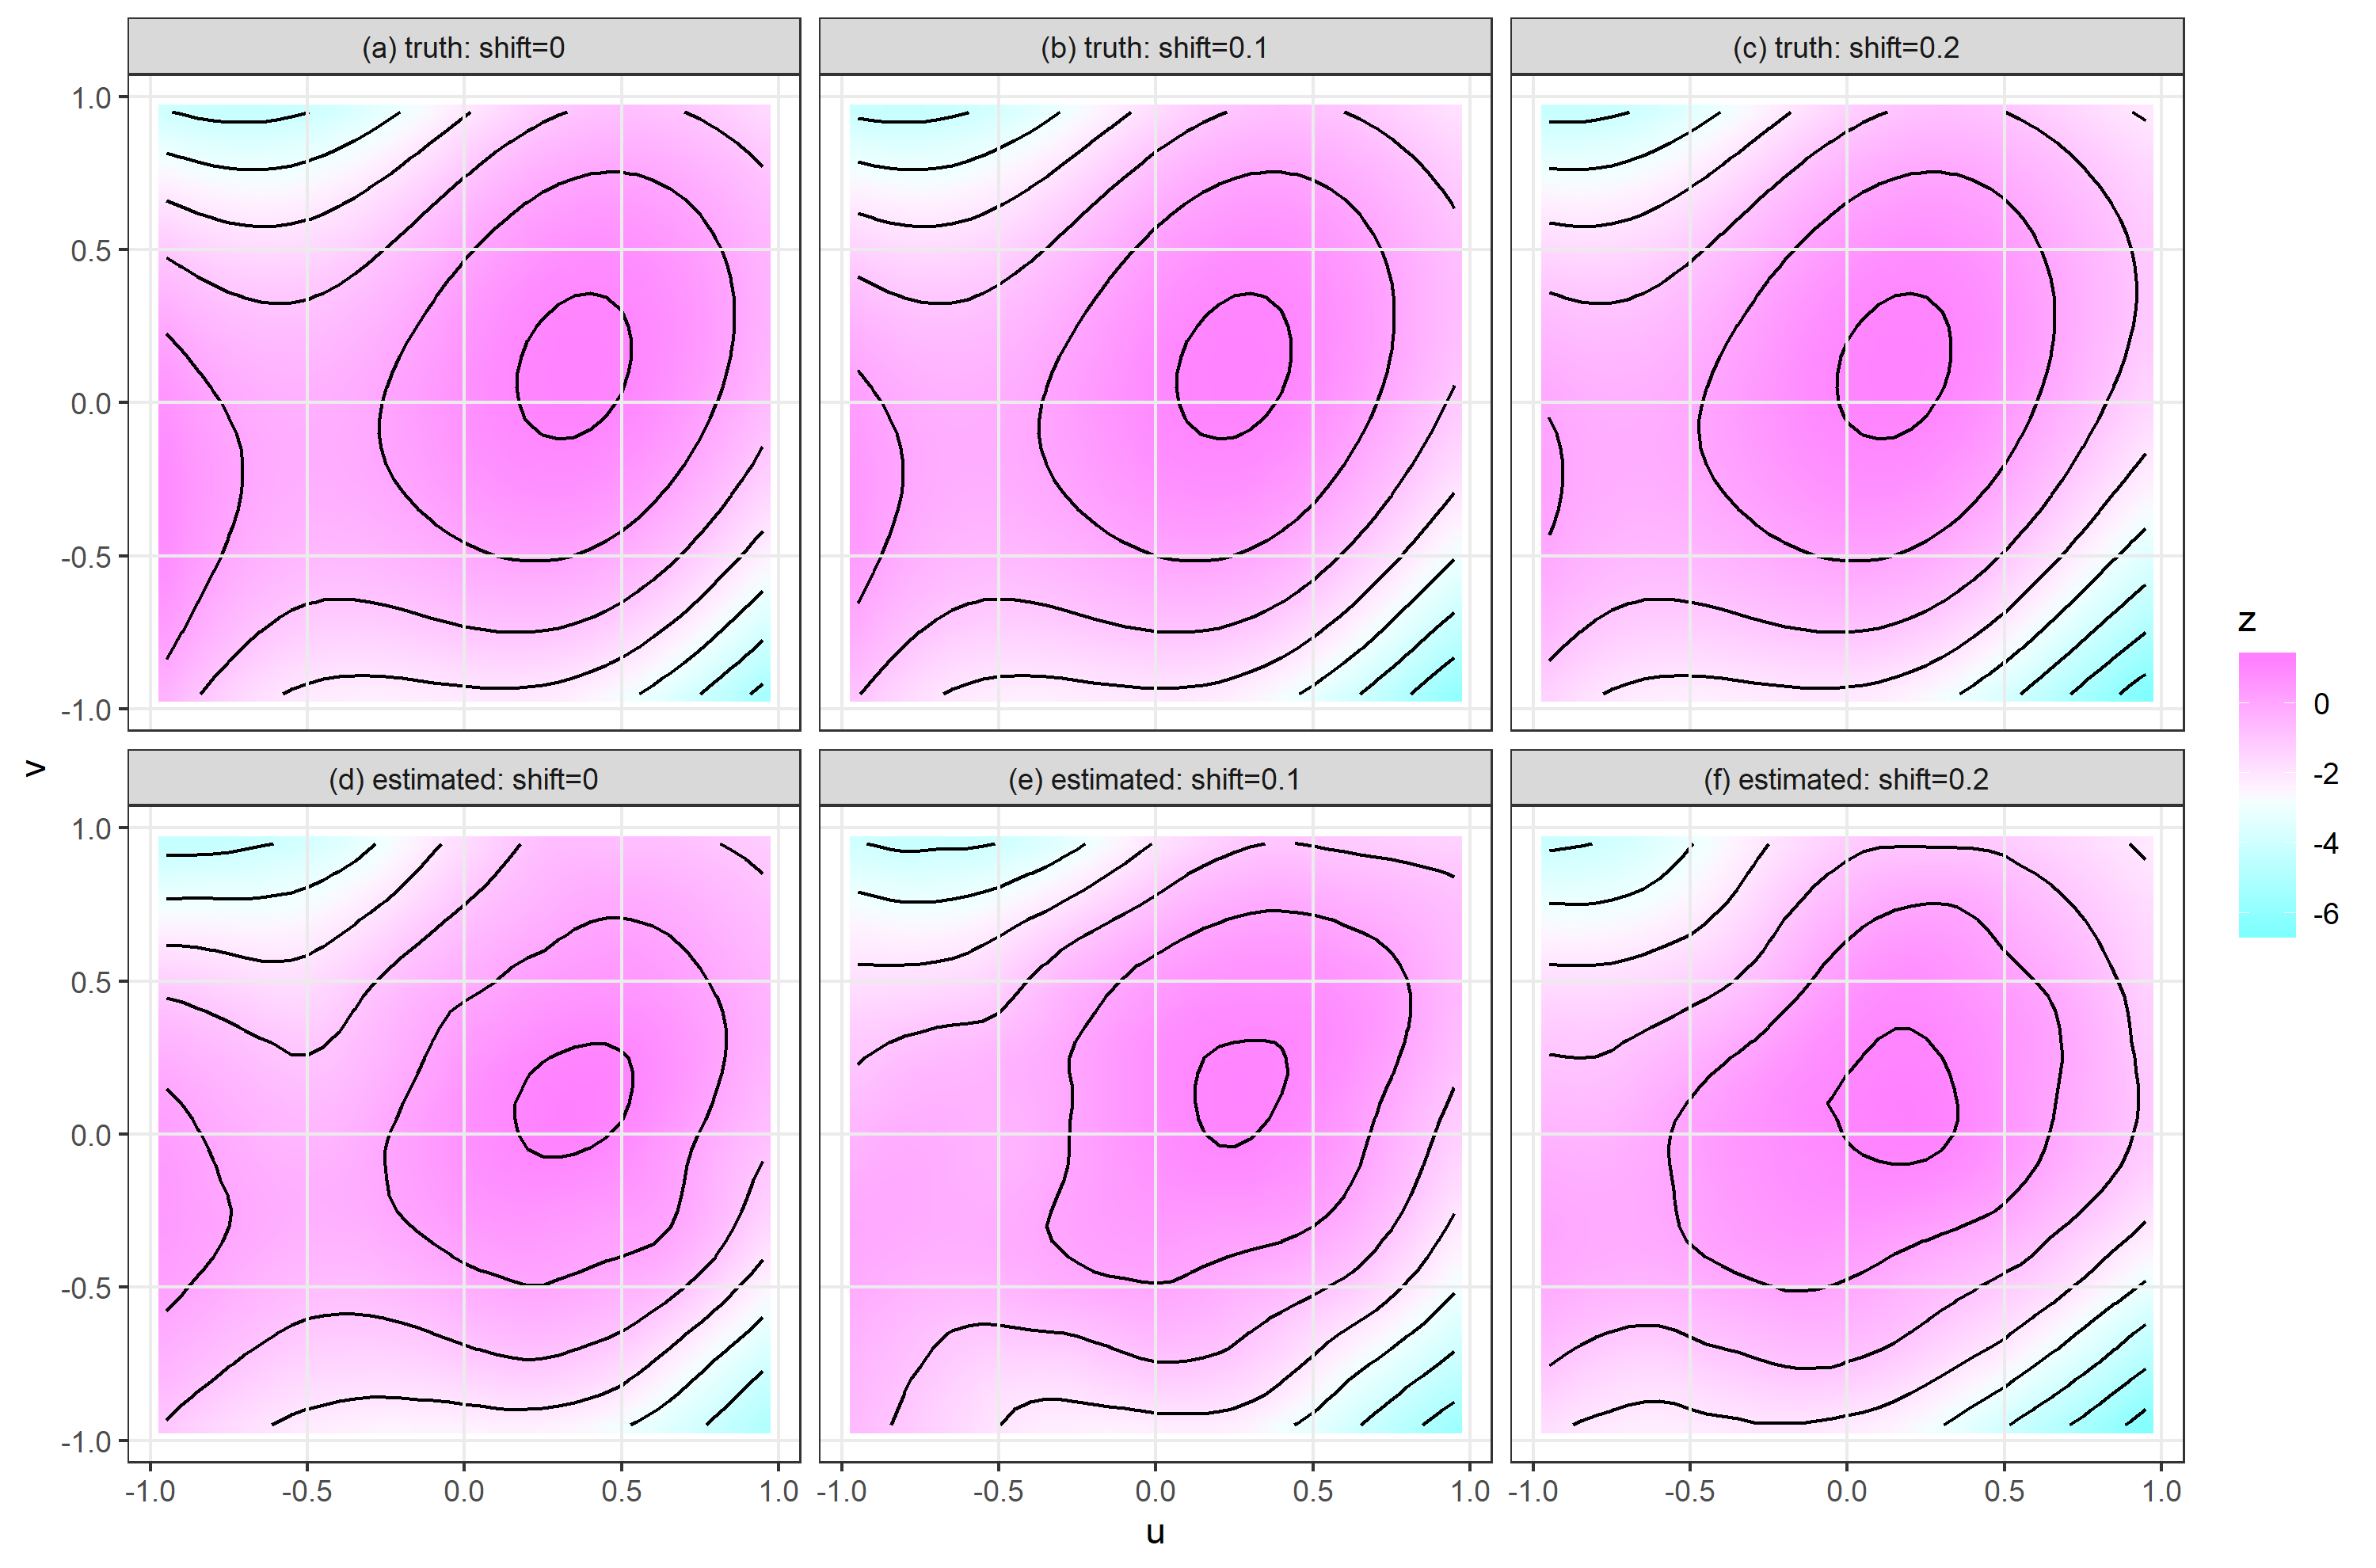
\includegraphics[width=\linewidth]{Figures/Chap3/TrueNEst.png}
		\caption{\textbf{Top}: Patterns used in nonlinear risk pattern simulations. ``shift" stands for the shifting amount of the whole pattern to left; \textbf{Bottom}: Estimated spatial risk patterns using our proposed model (in (\ref{stramodel})).}
		\label{fig:1}
	\end{figure}
	
	Using our proposed generalized additive model in (\ref{stramodel}), we are able to estimate the risk patterns at each time point. One simulation study is used to assess the performance of the stratified LOESS smoothers. 3 time points are set up with time-varying geospatial risk patterns where shift amounts are 0, 0.1 and 0.2, respectively. The 3 plots in the bottom of Figure \ref{fig:1} show the estimated risk patterns at each time point. From the plots, it is shown that the proposed time-specific LOESS smoothers are capable of recreating each of the time-specific geospatial risk patterns.
	
	Several simulations are conducted with 2 time points in total. Under $H_0$, we assume homogeneous underlying spatial effects ("shift=0") at both time points.  For simulations under $H_1$, "shift=0" is used for Time 1 and a shifted pattern is used for Time 2. The amount of shift indicates extremity of deviation from $H_0$, hence greater shift amounts should be detected with greater statistical powers. 
	
	Empirical powers are defined as the proportion of simulations in which $H_0$ is rejected. A level of significance of $\alpha=0.05$ is used. In each simulation scenario, simulation is repeated 500 times and $N_{perm}=1000$. As a comparison, we also consider ANOVA tests for temporal homogeneity in the above simulation settings when a naive parametric form of spatial effects is assumed. Specifically, consider Model (\ref{mod:ano1}) and and test $H_0: \beta_5=\beta_6=\beta_7=0$ using a permutation version of the F test. A permutation strategy is used in order to maintain a correct type I error. Specifically, for each simulated dataset, the permuted ANOVA procedure simply compares the observed F statistic and permuted F statistics, where the permuted F statistics are calculated using dataset with randomly permuted time labels. Also, the \emph{mgcv} package offers a class of stratified thin-plate regression splines and corresponding ANOVA tests. We applied this test as well for comparison. The resulting powers are shown in Panel (a) of Figure \ref{fig:twobtwo}.
	
	\begin{equation} \label{mod:ano1}
	E(Y_{ij}) =\beta_0+\beta_1u_{ij}+ \beta_2v_{ij}+\beta_3 t_{ij} + \beta_4 u_{ij} v_{ij} + t_{ij}(\beta_5u_{ij}+ \beta_6v_{ij}+\beta_7  u_{ij} v_{ij}) 
	\end{equation}
	
	To assess the performance of the PMSD test on datasets with more than 2 time points, we create datasets with 4 time points. No shift is used at time point 1 and a shift amount $S$ is applied at time point 4. For time 2 and 3, we used uniformly spaced shift amounts $S/3$ and $2S/3$. The resulting powers under these settings are shown in Panel (c) of Figure \ref{fig:twobtwo}. 
	
	\begin{figure}[h]
		\centering
		\includegraphics[width=\linewidth]{Figures/Chap3/Plot2b2XL1.png}
		\caption{\textbf{Panel (a)}: Power vs. shift amount based on 500 simulations at each shift value. Increasing rejection proportion could be observed. Type I error (rejection proportion at shift=0) is 0.046 for permutation test on F statistic, 0.032 for ANOVA F test based on thin-plate regression splines and 0.056 for PMSD test. The proposed PMSD test has the highest power in detecting temporal heterogeneity and permutation test based on parametric models renders the lowest power; 
			\textbf{Panel (b)}: Power vs. sample size based on 500 simulations at each sample size, given shift=0.15. Power increases along with sample size and approaches 1 near a sample size of 350 observations per time point; 
			\textbf{Panel (c)}: Power vs. shift amount at time point 4 based on 500 simulations at each shift value. Increasing rejection proportion (or greater power) could be observed. Type I error (rejection proportion at shift=0) is 0.062 for permutation test on F statistic, 0.018 for ANOVA F test based on thin-plate regression splines and 0.042 for PMSD test. Similarly, our proposed PMSD tests have better performance in power in detecting temporal heterogeneity;
			\textbf{Panel (d)}: Power vs. multiplier $\tau$ in (\ref{eq:paratruth}) based on 500 simulations at each value of $\tau$. As expected, classical ANOVA F test performs better in terms of power since it is the ``correct" test hence most powerful. In the meanwhile, the performance of PMSD is close to the F test.}
		\label{fig:twobtwo}
	\end{figure}
	
	The Monte Carlo results presented in Figure 2 for the PMSD test utilize a uniformly distributed $20\times 20$ grid on the entire $2\times 2$ map. Although a $20\times 20$ grid is seemingly sufficient for the risk patterns in the simulation studies we performed, we suggest a grid that is dense enough in order to sufficiently evaluate local behaviors. 
	% To explore the sensitivity of PMSD tests to the density of grid, we considered the impact of grid density on the performance of PMSD tests. Using simulation study, we evaluated a variety of grid densities for the PMSD test given a fixed shift amount 0.1. The corresponding power curve for each grid selection method is shown in Figure \ref{fig:gridpower}. These results suggest that too sparse a prediction grid hampers power, but simply choosing a higher density grid does not increase power to 1 (as it shouldn't). Note the distribution of the observed locations is uniform as well, 2 curves do not differ by much. 
	
	In addition to the grid density, another decision to make when performing PMSD tests is grid selection strategy. Intuitively, one might choose uniformly distributed locations on the entire map or the observed locations within the dataset. Since the MSD statistic is defined as the mean of squared differences at a chosen set of locations, the pattern of the grid intrinsically defines the weights assigned over the map. For temporal heterogeneity detection, a uniform grid will place equal weights on all areas of the map while observed locations put higher weight on areas with denser observations. As a simple example, given a risk pattern where temporal variation exists in one area of the map, using more points in the varying area in the grid for PMSD tests would result in higher power since the test would be weighted more heavily in the varying area due to the grid design. 
	
	To assess the impact of grid selection strategy on power, we performed simulation studies in 2 more scenarios. In Scenario 1 (shown in the plots in the top row of Figure \ref{fig:simuV2}), we use the same pattern as the previous simulations with 2 time points where we use "shift=0" for Time 1 and "shift=0.1" at Time 2. The observations are designed to be uniformly distributed on the map. We vary $N_g$, the number of locations used in the grid, to explore the impact of grid density on power. For each $N_g$ value, we simultaneously chose $N_g$ random locations from a uniform $20\times 20$ grid on the map and another random collection of $N_g$ locations from the observed location set. Using the 2 sets of locations, PMSD tests were performed in order to assess the impact of grid selection strategy on power. In Scenario 2 (bottom row of Figure \ref{fig:simuV2}), we use another design of spatial risk surface which has 2 high risk areas. We use the pattern at Time 1 and mitigate the risk by 30\% in one of the high risk areas at Time 2 to create temporal heterogeneity. In this setting, observations are designed to be denser in high risk areas. We performed similar grid selection and testing procedures to those of Scenario 1 and compared power with respect to grid density and selection strategy. From the empirical power results, the denser grids tend to render higher power, which is reasonable since local variations are more likely to be detected with more evaluated locations. In Scenario 1, tests using observed locations yield slightly higher power than those using uniform grids. This result could be explained by higher precision in spatial effects estimation at observed locations. The performance of tests using observed locations is much better than that of tests using a uniform grid in Scenario 2, which is as expected since more locations in time-varying areas are evaluated by MSD statistic, resulting in greater weights in the areas when the test is performed. 
	
	\begin{figure}[h] 
		\centering
		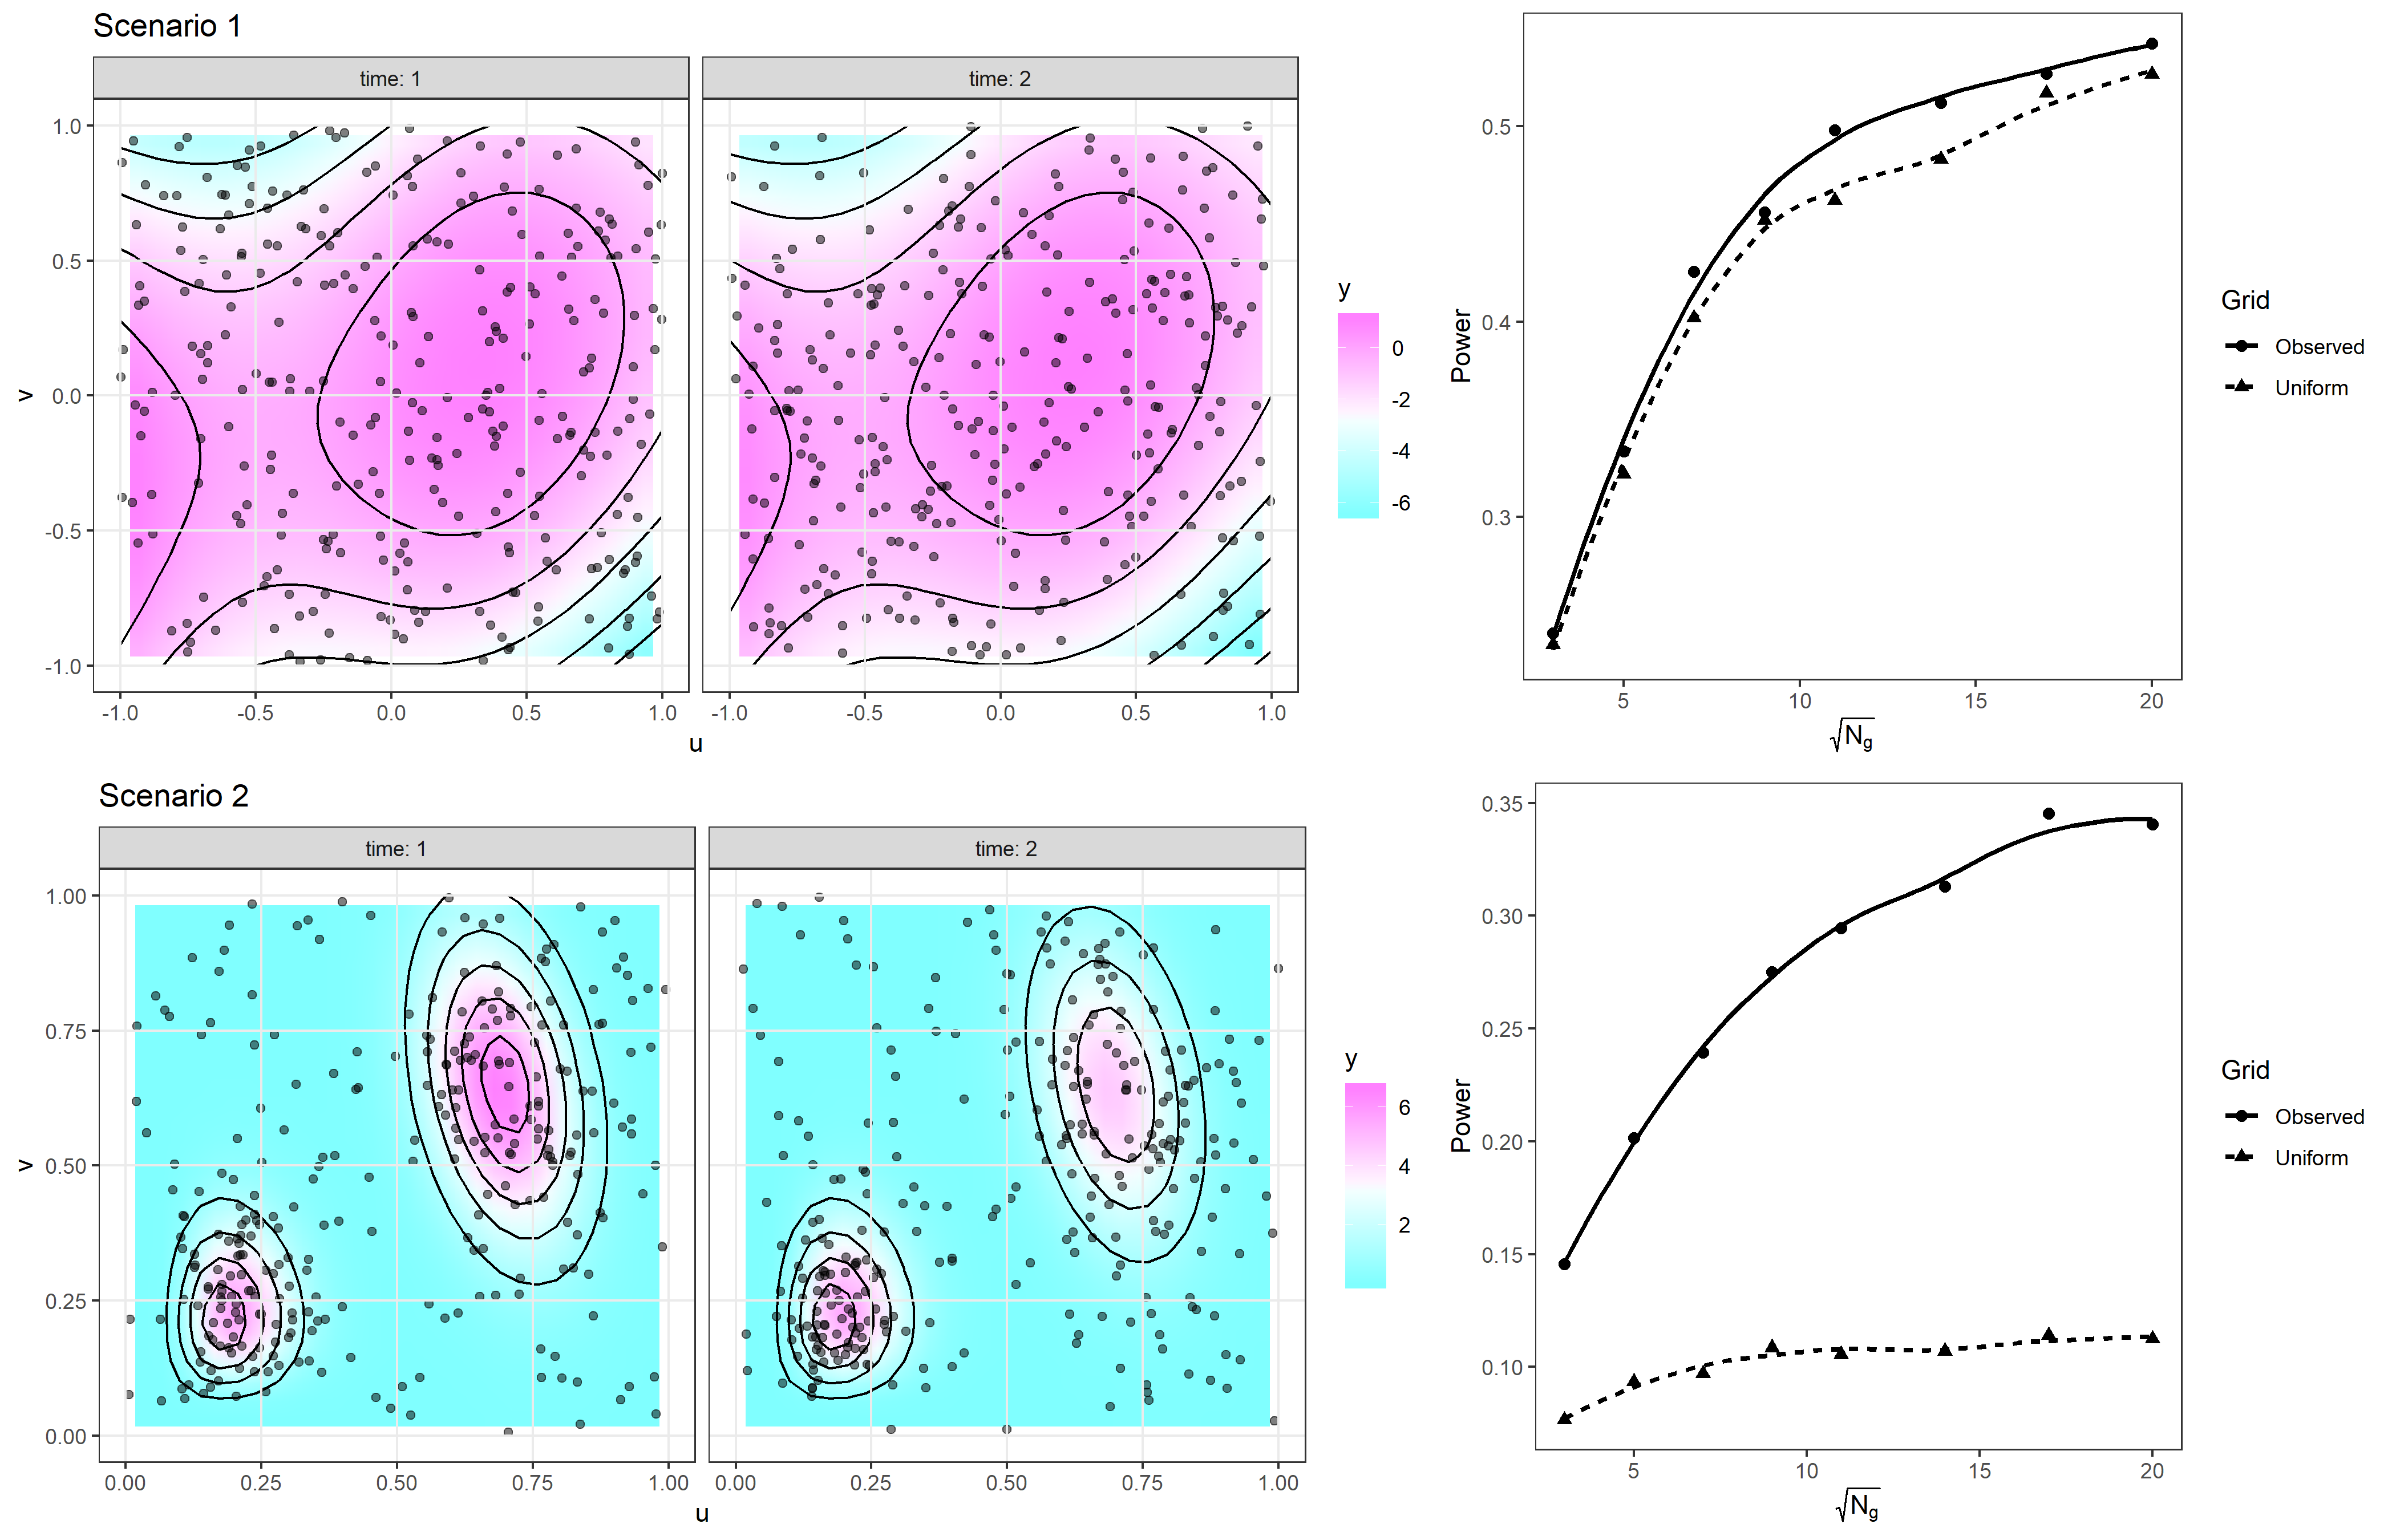
\includegraphics[width=\linewidth]{Figures/Chap3/gridc1234SNR.png}
		\caption{\textbf{Top}: Geospatial risk patterns at Time 1 and 2 with observed locations in Scenario 1 and corresponding power v.s. density curves for PMSD tests using uniform and observed grids. \textbf{Bottom}: Geospatial risk patterns at Time 1 and 2 with observed locations in Scenario 2 and corresponding power v.s. density curves for PMSD tests using uniform and observed grids.}
		\label{fig:simuV2}
	\end{figure}
	
	\subsection{Simulation studies with linear underlying patterns}
	
	In the previous Monte Carlo studies, we assume nonlinear underlying spatial patterns, as is shown in Figure \ref{fig:1}. In these situations, our proposed PMSD test outperformed a permutation version of the F test, as is expected. In this section, we conduct a simulation study where the true underlying spatial risk patterns are created using a linear function of longitude and latitude and compare the finite sample behavior of the PMSD tests and the optimal F tests.  Specifically, data were generated using the following model:
	\begin{equation}
	y_{ij}=-2+3u_{ij}-3v_{ij}+u_{ij}v_{ij}+\tau t_{ij}(2u_{ij}+2v_{ij}+u_{ij}v_{ij}+1)+\epsilon_{ij}.
	\label{eq:paratruth}
	\end{equation}
	
	In the above model, values from 0 to 0.16 are chosen to be $\tau$. $\epsilon_{ij}$'s are $i.i.d.$ random errors from a standard normal distribution. We apply both a classical ANOVA F test of the space-time interaction terms (a correctly specified model) and the PMSD test. Using a similar strategy as previous sections, we compare the performance of the 2 classes of tests and plot the results in Panel (d) of Figure \ref{fig:twobtwo}. Both tests yield correct type I errors while the ANOVA test yields slightly higher power. However, the increased power comes at a high cost, as the inflexible parametric model does not perform as well if the underlying risk pattern is more realistically nonlinear.
	
	\section{Application to birth defects study in Massachusetts}
	
	In this section we use our proposed methods to analyze the data achieved by the previously introduced MBDR study. Given the severity of PDA, it is of interest to determine if space-related risk factors place infants at increased PDA risk. Generalized additive models with a bivariate smoother incorporated, such as the model in (\ref{mod:orig}), estimate cross-sectional geospatial risk patterns with adjustment for other potentially relevant factors including maternal age, adequacy of prenatal care (measured by the Adequacy of Prenatal Care Utilization Index), maternal race, maternal education level and number of siblings, as is applied in  \cite{girguis2016maternal}. 
	
	Beyond the analysis of cross-sectional data in each year, we further aim to investigate the existence of variation in spatial risk patterns over time. We applied our methods on data collected in 2003, 2006, and 2009. Available sample sizes for the three years are 1082, 969, and 877, respectively. Corresponding numbers of PDA cases are 111(10.3\%), 90(9.3\%) and 60(6.8\%). The geographic distribution of the observations are shown in the top row of Figure \ref{fig:MAdist}. With adjustment for maternal age, adequacy of prenatal care, maternal race, maternal education level and number of siblings, the estimated geospatial risk patterns are shown in the bottom row of Figure \ref{fig:MAdist}. PMSD tests were performed to assess heterogeneity over the 3 years. The results are shown in Figure \ref{fig:MApvalues}. 
	
	\begin{figure}[h]
		\centering
		\includegraphics[width=\linewidth]{Figures/Chap3/obnest201904.png}
		\caption{\textbf{Top}: Distribution of PDA cases (red) and controls (black) over selected years. Sparsity in western Massachusetts reflects lower population density; \textbf{Bottom}: Estimated geospatial risks for each year with adjustment for relevant variables. Values presented are estimated log odds ratios. The solid lines on the estimated patterns indicate areas with significant nonzero log-odds using $\alpha=0.05$. The significance is determined by a permutation test described in \cite{webster2006method} The idea of the test is to randomly permute the locations of the observations and recalculate the log-odds for M times in order to achieve a point-wise reference distribution of log-odds at each point on map. The significant areas contain points where the estimated log-odds is outside of the 95\% confidence interval constructed by the reference distribution. The test is applied using R package \emph{MapGAM}. \citep{bai2019mapgam} According to the estimated surfaces, southeast Massachusetts has potentially significant high PDA risk in 2006 but low risk in both 2003 an 2009. In addition, a high PDA risk appears at central-southern Massachusetts in 2009.}
		\label{fig:MAdist}
	\end{figure}
	
	\begin{figure}[h]
		\centering
		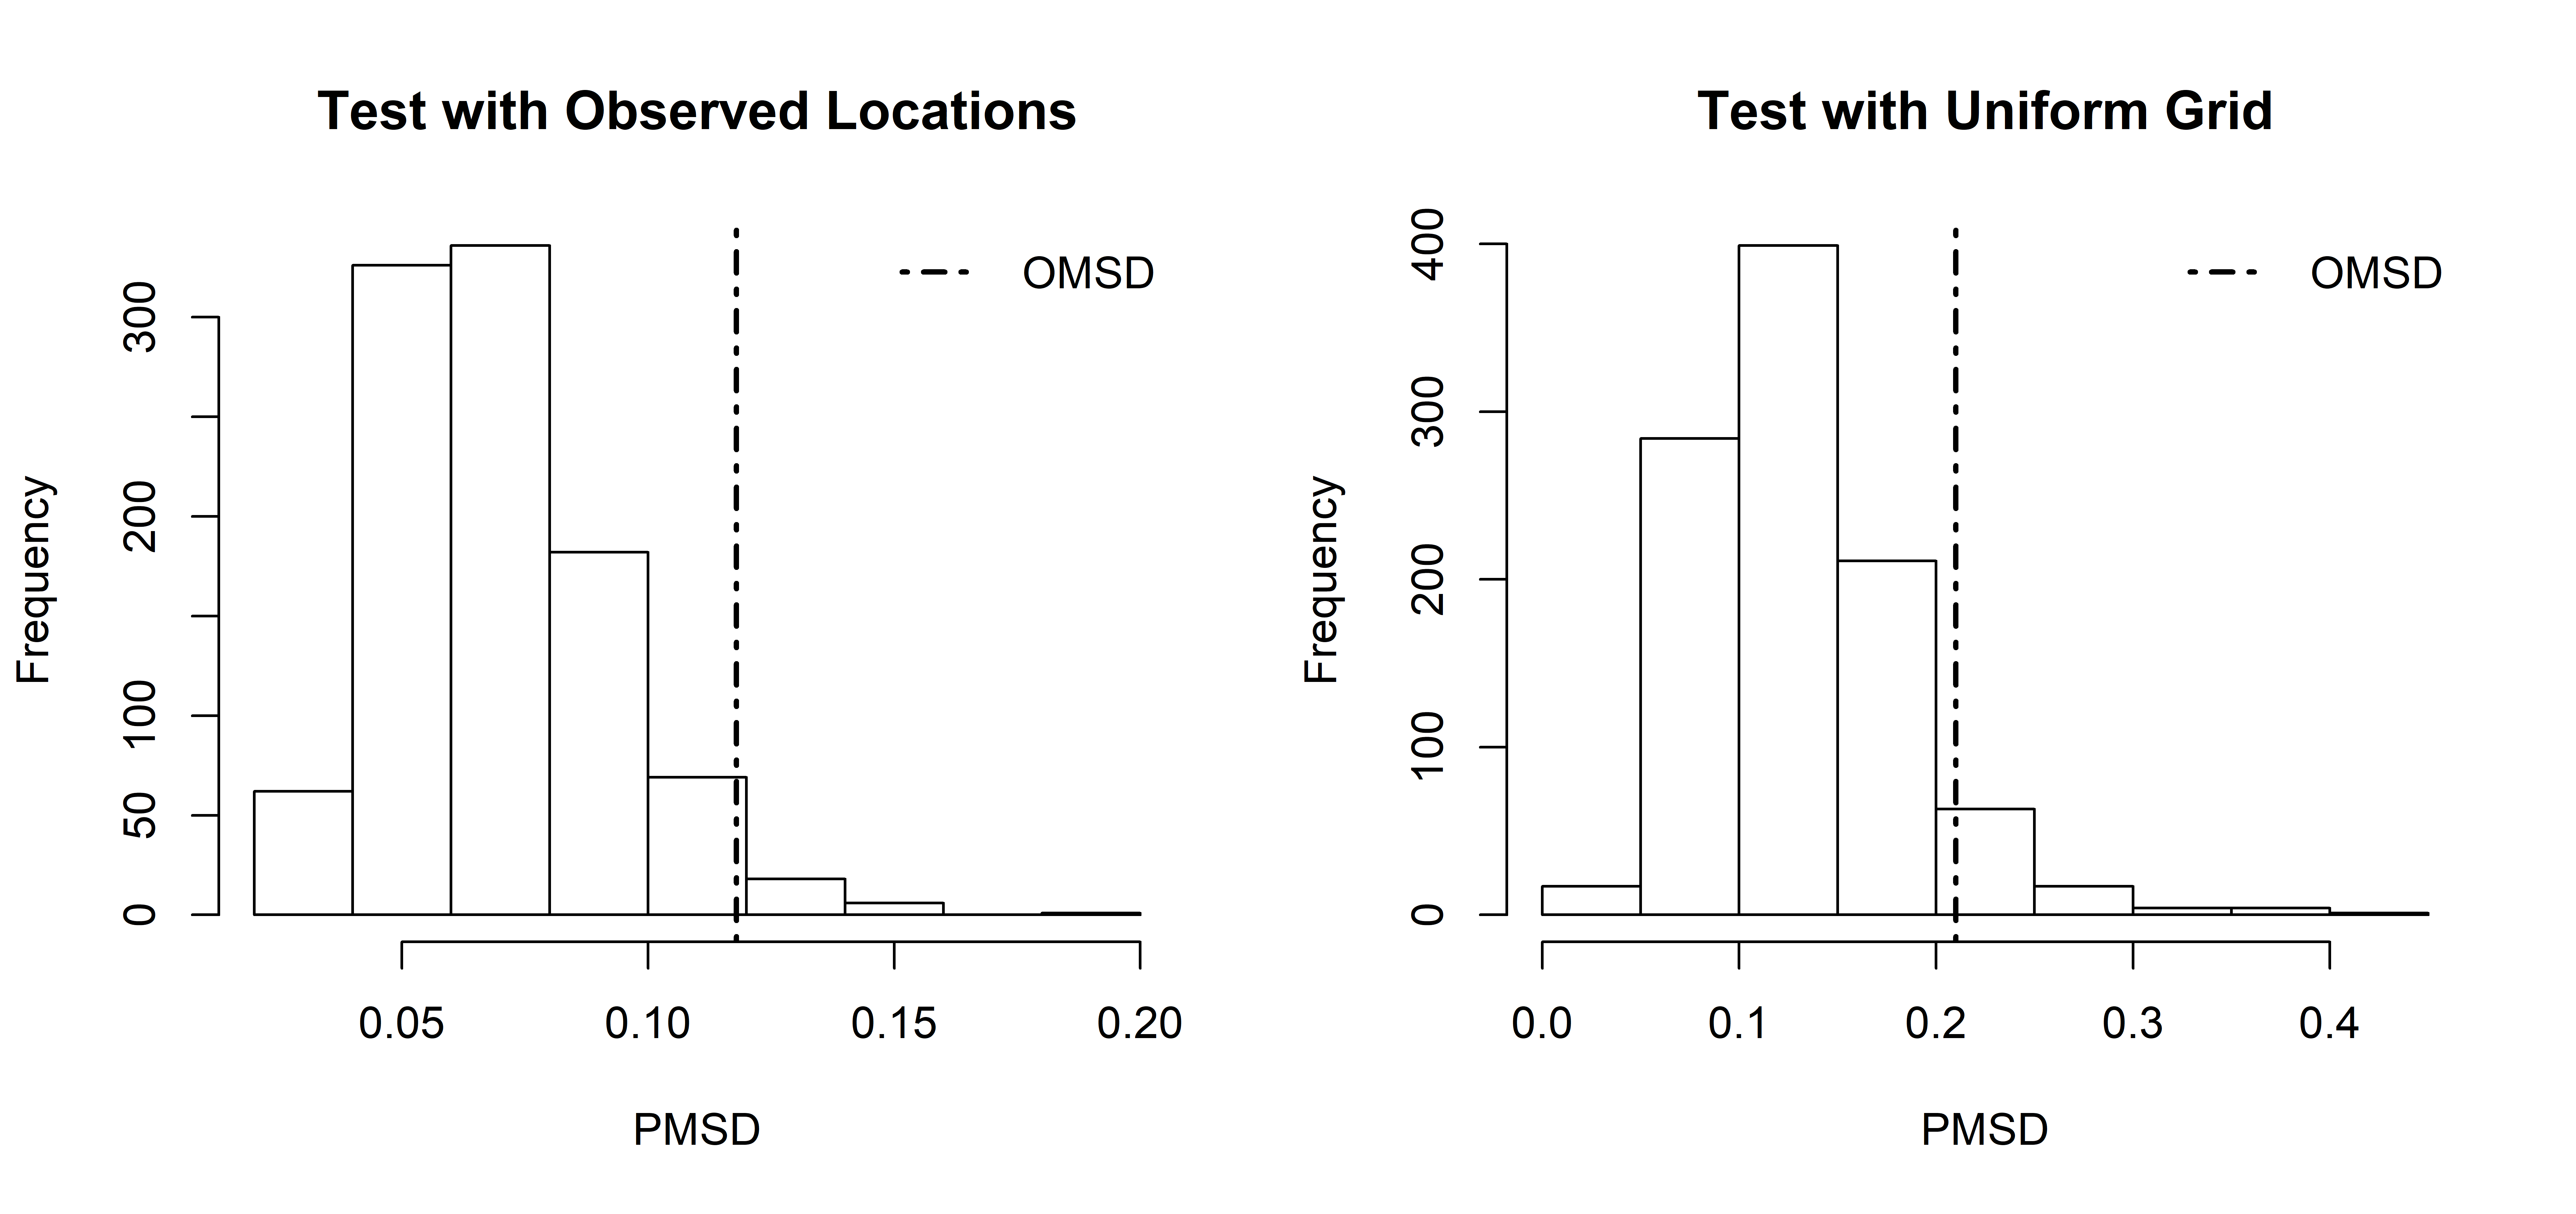
\includegraphics[width=0.9\linewidth]{Figures/Chap3/AppRes.png}
		\caption{Histograms of PMSD values using 2 test location selection strategies with vertical lines indicating the value of OMSD. The p-values are 0.029 using observed locations and 0.069 using a uniform grid on the Massachusetts map.}
		\label{fig:MApvalues}
	\end{figure}
	
	From the estimation in Figure \ref{fig:MAdist}, potential temporal heterogeneity of geospatial PDA risk is observed by visual inspection. To formally determine if the spatial risk changes over the period, we apply our proposed PMSD test and the resulting p-value is $0.028$, indicating potential time-varying and space-related factors for PDA risk other than the adjusted ones in the model over the 7 years from 2003 to 2009. Note that since the PMSD test aims to find any temporal change in the geospatial risk patterns, the detected heterogeneity could be a result of either a change in the overall level of PDA rate at each time point or a change in the spatial disparity patterns of PDA risk.
	
	The presented analysis utilizes all observed locations as evaluation points. The PMSD test utilizing a uniform grid on the Massachusetts map renders a greater p-value ($=0.069$) than the one using the observed locations (consistent with our previously presented simulation results). Corresponding PMSD and $\emph{OMSD}$ values are plotted in Figure \ref{fig:MApvalues}. As discussed previously, the choice between the two grid choice strategies should also take into account the scientific goals of the study. The PMSD test using observed locations places weights that are roughly proportional to the population (under a simple random sample) while the PMSD test using a uniform grid equally weights all areas of Massachusetts. 
	
	\section{Discussion}
	In this study, we brought in time-stratified kernel smoothers to the generalized additive model framework for estimation of time-specific geospatial disease risk patterns. Based on the proposed GAMs, we further formalized a permutation test for temporal heterogeneity of smoothed spatial risk effects.
	
	Using simulation studies, we showed that our proposed PMSD test performed substantially better than the other 2 competitors in detecting underlying temporal heterogeneity given a specific nonlinear spatial pattern. Even when the difference between spatial risk patterns was not clearly noticeable by visual inspection, the proposed procedure yielded acceptable power. In situations with parametric spatial risk patterns, a correctly specified parsimonious parametric ANOVA F test only slightly outperformed the PMSD test. We did assume smoothness of the surface in the presented simulations as well as smooth shifts over time as there would likely not be abrupt shifts in the spatial or temporal patterns for the birth defect data that motivates our methodology.  We do, however, acknowledge that non-smooth patterns can exist and differential changes in hot spots may arise. In additional simulation studies, not presented here, we considered the performance of our methods in the setting of abrupt changes in the response surface. We found that our model managed to render reasonably good estimation although the estimated pattern is not as accurate at the areas where the risk changes dramatically, which is not surprising since the smoothness assumption is violated. We also found that the type I error rate of our proposed PMSD test was maintained and that relative power benefits compared to the F test were also maintained in this setting. 
	
	Straightforward extensions of the proposed methods may be of interest in particular settings. For instance, if multiple contiguous time points are assumed to share one common spatial risk pattern, these time points could be grouped as one strata. Thus the stratified smoothers and corresponding PMSD tests are naturally applied to multiple time stratas, rather than to all time points. A similar strategy could be adopted for cases with continuous time, where smoothers could be stratified at separate time intervals. Also, when researchers wish to investigate heterogeneity in geospatial risk patterns over a categorical factor other than time, such as sex or discretized age, the proposed methods remain applicable. 
	
	The proposed PMSD test considers a global test for temporal homogeneity of spatial effects, as opposed to identification of specific local area differences. This is a natural first step in the identification of changing spatial patterns over time. Note that when temporal variation of geospatial risk pattern exists merely localized while the grid for MSD statistics is designed on the entire map, the power may suffer from the inclusion of geographic locations where the risk does not vary over the time period in MSD statistic. One next step, as we have done in the MBDR analysis for cross-sectional data analysis, is to highlight areas with differential risks. This is akin to first establishing the existence of main effects then further investigating effect modification. 
	
	Other than what is proposed in this work, smoothing with respect to time seems to be an intuitive way to model space-time data, but naively including time in smoothing terms is questionable. Using two separate smoothing terms in an additive way, one for spatial effects and another for time effects, fails to model time-space interaction while using a 3-way smoother including longitude, latitude and time offers flexible smoothing but suffers from anisotropy and potentially sparseness. The proposed procedures make no assumption on temporal correlation and put no restriction on how geospatial effects pattern varies. Some might be concerned about loss of efficiency due to the flexibility. We would argue that for large data sets, which is frequently the case in epidemiology studies, efficiency is maintained at each time point. As supporting evidence, Panel (d) of Figure \ref{fig:twobtwo} shows close performance between PMSD tests and the optimal ANOVA F-tests under parametric spatial risk patterns, indicating little efficiency loss.
	
	For statistical inference on smoothing components in GAMs, an approximate F-test was introduced by \cite{hastie1990generalized}. However, simulation studies showed that this approximate F-test renders inflated type I error in \cite{young2011generalized}. According to simulation results of the approximate F-test (not shown in this manuscript) on our simulation problem, inflated type I errors are observed as well. However, due to its efficiency potential, we will explore calibrating methods for this class of approximate F-tests in our future work. 
	
	An intuitive Bayesian counterpart of the stratified smoother could be a time-stratified Gaussian process where one process is set up at each time point with or without shared hyperparameters. A stratified Gaussian process only requires modification of the likelihood. This stratification does not require a specific time-space covariance structure since no specific temporal correlation is assumed. Based on this class of models, temporal heterogeneity in spatial patterns can potentially be tested using the Bayes factor.\citep{kass1995bayes} While we appreciate the Bayesian framework in geospatial modeling, many health researchers are not closely familiar with Bayesian methods.  In contrast, local linear regressions may be more intuitive and accessible to nonstatisticians. In particular, tuning a span size that is understandable as the proportion of data utilized in the local window of smoothing, is more straightforward than choosing hyperparameters in covariance structures of a Gaussian process. In addition, GP models tend not to scale well with respect to computation. In contrast, the time-stratified generalized additive models proposed here are computationally cheap and easily scale to large data sets. We compared model fitting time between GP models and GAMs using the R package \emph{spBayes} \citep{Finley2007, Finley2015} and R package \emph{gam} \citep{hastie1990generalized} respectively. GP models were roughly 20 times more computationally expensive when compared to GAMs for $N=100$. Computation times were roughly 200 times greater for $N=300$, 500 time greater for $N=500$ and 1000 greater for $N=700$, indicating a disadvantage of GP models with respect to scalability. Given these potential advantages, we view the proposed procedure as providing another useful tool to spatial epidemiologists.
	
	%In this paper, we assume simplistic homogeneous or heterogeneous risk patterns for our simulations, as well as independence over time conditional upon all adjustment covariates. Hence our method tests temporal homogeneity without assessing temporal correlation, and assumes no unmeasured confounding.
	
	One key assumption we made in this paper is mutual independence of all observations. That is to say, cross-sectional studies over multiple time points, rather than longitudinal studies, are discussed. Since longitudinal studies where individuals have multiple measurements over time are increasingly prevalent, in the future, we plan to further generalize stratified smoothers and investigate the performance of the PMSD tests on longitudinal data.
	


%%% Local Variables: ***
%%% mode: latex ***
%%% TeX-master: "thesis.tex" ***
%%% End: ***

%\chapter{Introduction}

In epidemiology studies, geospatial disparities of certain disease risks are of common interest since the potential unequal risks could be a result of location-related risk factors. These factors could be environmental, demographic, socioeconomic among others. Thus, spatial epidemiologists frequently aim to estimate a risk pattern over an area under study, which is frequently a residential geospatial area. 

This is an example using the \LaTeX{} template for UCI theses and
dissertation documents \cite{uci-thesis-latex}. Figure
\ref{fig:sourcecode} is just for illustration purposes, as is Table
\ref{tab:coordinates}.

\begin{figure}
\begin{verbatim}
#include <iostream>
int main(int argc, char** argv) {
  std::cout << "Hello World." << std::endl;
  return 0;
}
\end{verbatim}
  \caption{Example source code.}
  \label{fig:sourcecode}
\end{figure}

\section{Background}

Lorem ipsum dolor sit amet, consectetur adipisicing elit, sed do
eiusmod tempor incididunt ut labore et dolore magna aliqua. Ut enim ad
minim veniam, quis nostrud exercitation ullamco laboris nisi ut
aliquip ex ea commodo consequat. Duis aute irure dolor in
reprehenderit in voluptate velit esse cillum dolore eu fugiat nulla
pariatur. Excepteur sint occaecat cupidatat non proident, sunt in
culpa qui officia deserunt mollit anim id est laborum.

\begin{table}
  \centering
  \begin{tabular}{|rr|r|}
    \hline
    $x$ & $y$ & $z$ \\
    \hline
    14 & 12 & -2 \\
    0 & 33 & -25 \\
    -3 & 11 & 22 \\
    4 & 4 & 6 \\
    \hline
  \end{tabular}
  \caption{Example coordinates.}
  \label{tab:coordinates}
\end{table}

Lorem ipsum dolor sit amet, consectetur adipisicing elit, sed do
eiusmod tempor incididunt ut labore et dolore magna aliqua. Ut enim ad
minim veniam, quis nostrud exercitation ullamco laboris nisi ut
aliquip ex ea commodo consequat. Duis aute irure dolor in
reprehenderit in voluptate velit esse cillum dolore eu fugiat nulla
pariatur. Excepteur sint occaecat cupidatat non proident, sunt in
culpa qui officia deserunt mollit anim id est laborum.


%%% Local Variables: ***
%%% mode: latex ***
%%% TeX-master: "thesis.tex" ***
%%% End: ***

%\chapter{Generalized additive mixed models with kernel smoothers}
	
	\section{Introduction}
	\label{s:intro}
	% the problem of interest
	Geographically heterogeneous disease rates are of common interest in epidemiology studies since local high or low rates may serve as a surrogate for space-related risk factors such as environmental exposures and local healthcare access or quality. While traditional geographic modeling methods focus on analyzing aggregated area-level data that treat area-defined partitions as one unit, more recent spatial epidemiology studies avoid aggregation bias and the ecological fallacy by modeling individual-level data that may be collected longitudinally over time.  With accurate records of geospatial information (frequently longitude and latitude), researchers generally assume an underlying smooth surface for modeling the heterogeneity of disease risk over a given geospatial region, regardless of borders of inner areas. Based on this assumption, the estimation of the surface is an essential component in spatial data analysis. 
	
	Due to the complex nature of geospatial disease risk, it is not feasible to assume a parametric form to model the underlying risk surface in most cases. As such, nonparametric methods are popular in spatial effects modeling. Under a frequentist estimation framework, popular nonparametric methods include kernel and spline smoothers. Kernel smoothers utilize locally weighted models while spline smoothers are defined by a basis expansion of the design matrix over the full predictor support. In this work we consider locally weighted regression (LOESS) as proposed by \citet{cleveland1979robust}. LOESS assumes local (weighted) polynomial relationship between response and explanatory variables and was applied to geospatial analysis by \citet{brunsdon1996geographically} among others. One advantage of LOESS for spatial analyses is that it intuitively adapts to changing population densities by varying the size of the smoothing neighborhood based on the local data density given a fixed span size (typically defined as the proportion of observations used for local regressions). %One popular way to choose an optimal span size is to use Akaike information criterion (AIC). \citep{akaike1998information}
	
	In addition to spatial risk pattern estimation, confounding variables, such as biomarkers in studies on public health, should be included in spatial models. Generalized additive models (GAMs) \citep{hastie1990generalized} offer a framework for incorporating frequentist smoothers and confounding variables in an additive fashion by assuming a linear predictor consisting of the sum of nonparametric smoothers and parametric adjustment covariates. \citet{wood2017generalized} further developed GAMs by incorporating various types of splines and covered relevant topics such as computation, properties and applications. 
	
	% From GAM to GAMM
	In recent years, data collection methods such as patients revisits and health trackers have become increasingly prevalent. These procedures frequently result in multiple longitudinal measurements on individuals over time. This sampling framework results in within-subject correlation that must be accounted for in analytic methods in order to provide valid inferential results. As one example, a fairly recent study was conducted to investigate serum perfluorooctanoic acid (PFOA) concentration among residents in Lubeck, West Virginia and Little Hocking, Ohio. \citep{bartell2010rate} In this study, researchers aimed to understand the declining behavior of PFOA concentration after granular activated carbon filtration on the public water systems in 2007. By design, 200 residents were included and 6 blood samples were to collect from each resident from May 2007 to August 2008 so that a trend of PFOA concentration could be observed. Besides PFOA concentration, residents' information such as gender, age and recent water consumption type (public water or bottled water) was recorded as well as precise residential location (recorded as longitude and latitude). One of the objectives is to understand the geospatial distribution of residents' serum PFOA concentration in order to help identify potential latent space-confounded risk factors. 
	
	To account for within-subject correlation, random effects that account for individual-level effects are commonly adopted. \citet{breslow1993approximate} described a class of generalized linear mixed models (GLMMs) that incorporate linear predictors and random effects for modeling exponential family outcome variables, along with approximate fitting procedures to fit GLMMs. Based on GLMM and GAM, \citet{lin1999inference} proposed generalized additive mixed models that incorporate fixed effects, random effects and spline smoothers in order to estimate flexible function and confounding effects simultaneously with adjustment of within-subject correlation. Alternatively, \citet{Tang2020Additive} proposed a class of additive mixed models (AMMs) with kernel smoothers for disease mapping given Gaussian distributed outcome variable. However, to the best of our knowledge, no existing literature covers GAMMs with kernel smoothers. To fill this gap, this manuscript seeks to incorporate kernel smoothers and random effects into a generalized linear model and propose the corresponding model fitting and inference methods. This work could be viewed as a direct generalization of \citet{Tang2020Additive} with accommodation of more generally distributed outcomes. 
	
	The remainder of the manuscript is organized as follows: In Section 2, we introduce our proposed GAMMs and the corresponding model fitting procedure. In Section 3, we present simulation studies designed to assess the performance of our new model in geospatial risk pattern recreation and parameter estimation. In Section 4, we applied our proposed methods on PFOA data to estimate the geospatial pattern in serum PFOA concentration in the area of Lubeck, WV. Lastly, Section 5 provides further discussion about the proposed work and considers avenues of future research.
	
	\section{Methods}
	\label{s:Methods}
	\subsection{Notations}
	Let $i=1,2,\dots,N$ be the individual index where each $i$ corresponds to one individual. For each individual $i$, measurements are taken at times $t_{i1}, t_{i2},\dots,t_{iJ_i}$. The exponential family outcome of individual $i$ is denoted with a response vector $y_i=(y_{i1}, y_{i2}, \dots, y_{iJ_i})$. $x_{ij}$ stands for a length-$p$ vector of confounding variables of individual $i$ at time $t_{ij}$. In addition, each individual's geographical information (i.e. longitude and latitude) is tracked, labeled by $(u_{ij},v_{ij})$. %Independence is assumed among individuals but not among the repeated measurements within each individual in statistical analysis.
	
	%  Let $j=1,\dots,J$, denote a discrete time index and $i=1,\dots,N$, denote the individual index. Let $Y_i=(y_{i1}, y_{i2}, y_{i3}, \dots, y_{iJ})$ denote the vector of continuous responses for individual $i$.  We assume independence between individuals while allowing for correlation between measurements on the same individual. In addition, we note that $Y_i$ does not need to be complete with length $J$. In other words, individuals might not be measured at all time points. Let $(u_{i},v_{i})$ denote the geospatial location (longitude and latitude) of observation $i$ across all time, and let the function $lo()$ denote a LOESS smoother. Finally, let $X_{ij}$ denote a length-$p$ vector of potential time-dependent adjustment variables corresponding to observation $i$ at time $j$. 
	
	\subsection{Generalized additive mixed models with kernel smoothers}
	
	Starting with generalized linear models (GLMs, \cite{mccullagh2018generalized}), in this section we provide brief introduction to the formation of generalized additive models (GAMs, \cite{hastie1990generalized}) and generalized linear mixed models (GLMMs, \cite{breslow1993approximate, wolfinger1993generalized}). We will then propose our noval class of generalized additive mixed models (GAMMs) by combining GAMs and GLMMs. 
	
	Generalized linear models are virtually the most popular regression models when an exponential family outcome variable, such as a binary outcome or a counting outcome, is of interest. Specifically, GLMs assume that the outcome $y_i$ follows a distribution of exponential family with $E(y_i)=\mu_i$ and $\text{var}(y_i)=v(\mu_i)$, where function $v()$ depends on the specific distribution of $y_{i}$. Commonly seen distributions of response $y_i$ include Gaussian, Bernoulli and Poisson among others. The mean $\mu_i$ is linked to the linear predictor $x_i^T\beta$ by the link function $g()$. Hence a GLM is commonly written as 
	\begin{equation}\label{mod:GLM}
	g(\mu_i)=x_{i}^T\beta. 
	\end{equation}
	GLMs generally assume independence among data hence are appropriate in cross-sectional studies where linearity suffices to model the relationship between $g(\mu_i)$ and  the explanatory variables $x$. 
	
	If the independence assumption is released in GLMs by inducing random effects $b_i$ to model cluster-specific effects, the linear predictor is then written as
	\begin{equation}\label{mod:GLMM}
	g(\mu_{ij})=x_{ij}^T\beta + z_{ij}b_i, 
	\end{equation}
	where $b_i \stackrel{i.i.d.}{\sim} \text{MVN}(0,D(\theta))$ and $D(\theta)$ is the variance-covariance matrix as a function of parameter vector $\theta$. Due to the inclusion of the random effects $z_{ij}b_i$, this resulting model (Model (\ref{mod:GLMM})) is then named generalized linear mixed model (GLMM). 
	
	Other than GLMM, another class of generalization of GLM is achieved by release the linearity assumption. Specifically, smooth functions $s_k()$'s are used to replace all or part of the linear terms hence in general, the mean model becomes
	\begin{equation}\label{mod:GAM}
	g(\mu_i)=\sum_{k=1}^p s_k(x_i), 
	\end{equation} 
	which is then intuitively named as a generalized additive model (GAM) since arbitrary functions $s_k()$'s are combined in an additive fashion.
	
	As is mentioned in Section 1, since we aim to build a class of models that accommodate exponential family response, random effects and smoothers simultaneously, combination of GLMM and GAM would be a natural approach. Altervatively stated, we are interested in a class of models with a mean function\begin{equation} \label{mod:GGAMM}
	g(\mu_{ij})=\sum_{k=1}^p s_k(x_{ij}) + z_{ij}^Tb_i.
	\end{equation} 
	Specifically, since we develop our methods initially for disease mapping in geospatial epidemiology studies and our collaboration group prefer kernel smoothers (LOESS smoother in particular) for spatial risk pattern estimation, the mean model of direct interest could be written as
	\begin{equation} \label{mod:GAMMKernel}
	g(\mu_{ij})=x_{ij}^T\beta + lo(u_{ij}, v_{ij}) + z_{ij}^Tb_i,
	\end{equation} where $x_{ij}^T\beta$ models confounding effects, $lo(u_{ij}, v_{ij})$ models a flexible underlying spatial effects on the target disease risk and $z_{ij}^Tb_i$ ($b_i \stackrel{i.i.d.}{\sim} \text{MVN}(0,D(\theta))$) stands for individual-specific random effects, such as random intercepts or random slopes. 
	
	\subsection{Model fitting Procedure} \label{s:fitting}
	As we stated in Section 1, although \cite{lin1999inference} proposed a neat double penalized quasi-likelihood (DPQL) fitting procedure and approximate inference which considered both random effects and smoothing terms as penalization when maximizing likelihood of the full model for GAMMs with spline smoothers only, it was also recognized in their work that kernel smoothing was not accommodated due to the fact that kernel smoothers are generally not trivially parametrizable. Since we, along with our collaborators who are epidemiologists, prefer LOESS, which is essentially a commonly used type of kernel smoothers, for disease risk mapping in GAMMs, we would fill the gap and propose the fitting and inference methods for GAMMs with kernel smoothers in this section and LOESS would be focused on.
	
	Since we will build our algorithm based on the penalized quasi-likelihood (PQL) method for GLMMs, it would be beneficial to first introduce the application of PQL method before we elaborate the fitting procedure for our proposed class of GAMMs. To fit a GLMM, \cite{breslow1993approximate} provided PQL method to produce efficient inference and \cite{wolfinger1993generalized} further elaborated the computation in a more detailed fashion. In practice, the PQL estimation is achieved using an iterative strategy. In particular, when a GLMM, say Model (\ref{mod:GLMM}), is to be fitted, working response $y_{ij}^w$ is defined as
	\begin{equation} \label{eq:workingresponse}
	y_{ij}^w=g(\hat{\mu}_{ij})+(y_{ij}-\hat{\mu}_{ij})g^\prime(\hat{\mu}_{ij}),
	\end{equation}
	with reasonably initialized $\hat{\mu}_{ij}$. The working response vector $\mathbf{y}_{\hat{\mu}}^w$ could then be approximated by a Gaussian distribution 
	\begin{equation} \label{eq:ApproxGauss}
	N[X\beta+Zb,\ g^\prime(\hat{\mu})R_{\hat{\mu}}  g^\prime(\hat{\mu})],
	\end{equation} 
	where $R_{\hat{\mu}}$ is the variance-covariance matrix defined by the assumed outcome distribution given the estimated mean vector $\hat{\mu}$. It follows that a weighted linear mixed model 
	\begin{equation} \label{mod:workingLME}
	\mathbf{y}_{\hat{\mu},ij}^w=x_{ij}^T\beta+z_{ij}b_i+\epsilon_{ij}
	\end{equation}
	with working diagonal weight matrix 
	\begin{equation} \label{eq:W}
	\hat{W}_{\hat{\mu}}=R_{\hat{\mu}}^{-1}[g^\prime(\hat{\mu})]^{-2}
	\end{equation} 
	could be used to model the working response $\mathbf{y}_{\hat{\mu}}^w$. The PQL estimating procedure iteratively fits weighted linear mixed model with updated working response $\mathbf{y}_{\hat{\mu}}^w$ and working weight matrix $\hat{W}_{\hat{\mu}}$ based on the updated $\hat{\mu}$ at each iteration until the difference in parameter estimations are sufficiently small. 
	%For canonical link function $g()$, $\hat{W}=R_{\hat{\mu}}$. 
	
	Based on the PQL procedure, \cite{lin1999inference} developed double penalized quasi-likelihood (DPQL) by incorporating spline smoothers into GLMM framework with an additional penalization term to control the smoothness of the smoothers. However, while spline smoothing could be achieved by using basis expansion functions of the design matrix, kernel smoothing could not be achieved in such ways. Consequently, in order to fit a GAMM with kernel smoothers, such as Model (\ref{mod:GAMMKernel}), under PQL framework, weighted additive mixed models with kernel smoothers, instead of weighted linear mixed models in a classic GLMM framework, need to be fitted at each iteration. To fit this class of additive mixed models (AMMs), we refer to the framework proposed by \cite{Tang2020Additive}. 
	
	\cite{Tang2020Additive} provided a class of additive mixed models with kernel smoothers for Gaussian response and elaborated the novel fitting procedure for the class of model in detail. As a brief summary, They used a modified backfitting algorithm which performed a linear mixed model and a variance-covariance adjusted kernel smoother iteratively until convergence. That is to say, their algorithm iteratively updates the estimation of spatial effects and other parameters by fitting the partial residuals. One prudent contribution of theirs was a procedure to adjust for the estimated variance-covariance information when fitting a kernel smoother. Under the derivation that the working response $\mathbf{y}_{\hat{\mu}}^w$ is approximately Gaussian (see \ref{eq:ApproxGauss}), their method serves as a suitable choice when we want to fit the working response at each iteration within a PQL fitting procedure. 
	
	To summarize, with the combination of the classic PQL procedure by \cite{wolfinger1993generalized} and the algorithm for additive mixed models by \cite{Tang2020Additive}, a model fitting procedure for our proposed GAMM (Model (\ref{mod:GAMMKernel})) could be sketched as 
	
	\begin{enumerate}
		\item initialize $\hat{\mu}$ using a GAM $g(E(y_{ij}))=x_{ij}^T\beta+lo(u_{ij},v_{ij})$
		\item update working response $\mathbf{y}_{\hat{\mu}}^w$ using Eq. \ref{eq:workingresponse} and working weight matrix $\hat{W}_{\hat{\mu}}$ using (\ref{eq:W}) with the updated $\hat{\mu}$
		\item fit the working response with AMM ${y}_{\hat{\mu},ij}^w=x_{ij}^T\beta + lo(u_{ij}, v_{ij}) + z_{ij}^Tb_i+\epsilon_{ij}$ with weight matrix $\hat{W}_{\hat{\mu}}$, rendering inference on model parameters (including $\hat{\mu}$
		\item repeat Step 2 and 3 until the difference in estimated parameters between iterations are satisfyingly small. 
	\end{enumerate}
	
	Estimation and inference of the model parameters would be achieved from the final version of the working AMM. Since backfitting algorithm is adopted, inference on $\beta$ and $\theta$ would be achieved from the classic linear mixed model theory using ML or REML while inference on spatial effects would be based on the kernel smoother. Specifically, using the local model, the estimated spatial effect at a specific location $(u^*,v^*)$ could be written as 
	\begin{equation} \label{eq:haty}
	\hat{lo}(u^*,v^*)=H^*(\hat{\theta})y^*,
	\end{equation}
	where $H^*(\hat{\theta})$ stands for the estimated variance-covariance adjusted local hat matrix and $y^*$ would be the corresponding local partial residuals. Using a similar strategy as in \citet{Tang2020Additive}, the variance of $\hat{lo}(u^*,v^*)$ could be estimated by
	\begin{equation} \label{eq:VarLO}
	\widehat{Var}(\hat{lo}(u^*,v^*))=H^*(\hat{\theta})\widehat{Var}(Y^*)H^{*T}(\hat{\theta}).
	\end{equation}
	
	\subsection{Out-of-sample likelihood for smoothing parameter selection}
	
	Under most smoothing framework, choosing the right amount of smoothing is vital to avoid potental over-smoothing or under-smoothing. Popular smoothing techniques in disease mapping, such as a popular spline approach thin-plate splines \citep{wood2003thin} and a popular kernel approach LOESS \citep{cleveland1979robust}, use one parameter to control the smoothness of the estimated surface. Since we focus on LOESS smoother, we would mainly pay our attention to span size, the smoothness parameter for LOESS. As is commonly known, LOESS approach uses local weighted linear models to achieve a nonparametric estimation of the underlying risk surface. Span size (or span for short) indicates the proportion of data used in the local models. Partially due to the fact that LOESS, like most of other kernel smoothers, could not be fitted using basis expansion of the covariates, smoothing parameter could not be integrated into a unified likelihood expression, unlike most spline smoothers. 
	
	Similar to model selection in general, span is commonly chosen according to criteria such as AIC and GCV. \cite{Tang2020Additive} used AIC for span choosing and achieved satisfying results. However, based on the results from simulation studies in multiple synthesized scenarios, AIC does not have a stable performance in span selection for our proposed GAMMs. Conditional AIC, also known as cAIC, by \cite{vaida2005conditional} were tested as well but no satisfying span selection was observed.
	
	The reason for the failure of AIC and cAIC in span selection could partially be due to the fact that the degree of freedom used by the LOESS smoother could merely be approximated by the trace or similar metrics of the hat matrix. When the outcome follows an arbitrary exponential family distribution, we end up with decreased information from data, compared to Gaussian distributed outcomes, resulting in inaccurate estimation of smoother degree of freedom.
	
	In this section, we will propose an out-of-sample likelihood Monte Carlo (OLMC) method for smoothing parameter selection. We first randomly divide the sample in 2 subsets: a training set $\mathbf{y}^{(t)}$ and a validation set $\mathbf{y}^{(v)}$. Since observations from one individual or cluster would commonly be correlated, the randomization should be performed based on individuals rather than observations. In other words, no individuals should have measurements in both training and validation sets. Given candidate span values, we further train our GAMM, achieve the estimated fixed effects ${\hat{\beta}}^{(t)}$, estimated LOESS smoother ${\hat{lo}}^{(t)}$ and variance-covariance component $\hat{D}^{(t)}$. Based on the trained model, we aim to calculate the likelihood of the validation set using 
	\begin{equation} \label{eq:OoOl}
	\begin{split}
	L_{v|t}  &= p_1(\mathbf{y}^{(v)}|{\hat{\beta}}^{(t)}, {\hat{lo}}^{(t)}, \hat{D}^{(t)}) \\
	&= \int p_1(\mathbf{y}^{(v)}|{\hat{\beta}}^{(t)}, {\hat{lo}}^{(t)}, b^{(v)})p_2(b^{(v)}|\hat{D}^{(t)}) db^{(v)},
	\end{split}
	\end{equation}
	where $p_1()$ stands for the likelihood of the response (from an exponential family), $p_2()$ is the likelihood of the random effects (from a Gaussian distribution $N(0,\hat{D}^{(t)})$), $b^{(v)}$ stands for the corresponding individual-level random effects. 
	
	It worth noticing that the integral in Equation (\ref{eq:OoOl}) is not tractable, so we recommend a Monte Carlo method with a simulated sample of $b^{(v)}$. In particular, we simulate a relatively large sample (we used 500 in this work) from $N(0,\hat{D}^{(t)})$, use the each drawn sample $b^{(v), (k)},\ k=1,\dots,500$, to calculate the likelihood using 
	\begin{equation} \label{eq:p1k}
	p_1^{(k)}=p_1(\mathbf{y}^{(v)}|{\hat{\beta}}^{(t)}, {\hat{lo}}^{(t)}, b^{(v),(k)})
	\end{equation}
	and then calculate the Monte Carlo approximation of $L_{v|t}$ using 
	\begin{equation} \label{eq:MCL}
	L_{v|t}^*= \underset{k}{\text{mean}}\ p_1^{(k)}.
	\end{equation}
	
	This out-of-sample likelihood Monte Carlo approach provides a efficient and convenient evaluation of the model's out-of-sample performance hence when comparing the proposed GAMMs with differing span sizes, it is advisable to choose the model with the greatest $L_{v|t}^*$ value since greater out-of-sample likelihood generally indicates less amount of over-fitting or under-fitting of the spatial effects when span is the only varying factor. 
	
	\section{Monte Carlo studies}
	To assess the performance of our proposed model, we conducted multiple simulation studies based on a $2\times 2$ square map with a true spatial pattern given by
	\begin{equation}\label{eq:nlsim}
	s_0(u,v) =1.7+0.25[1.2\sin(3u+0.3)+2uv+ 6\log(0.6)v^2]
	\end{equation}
	and depicted in the Figure \ref{f:trueSpatial}. 
	
	% Figure 1 here
	\begin{figure}[h]
		\centering
		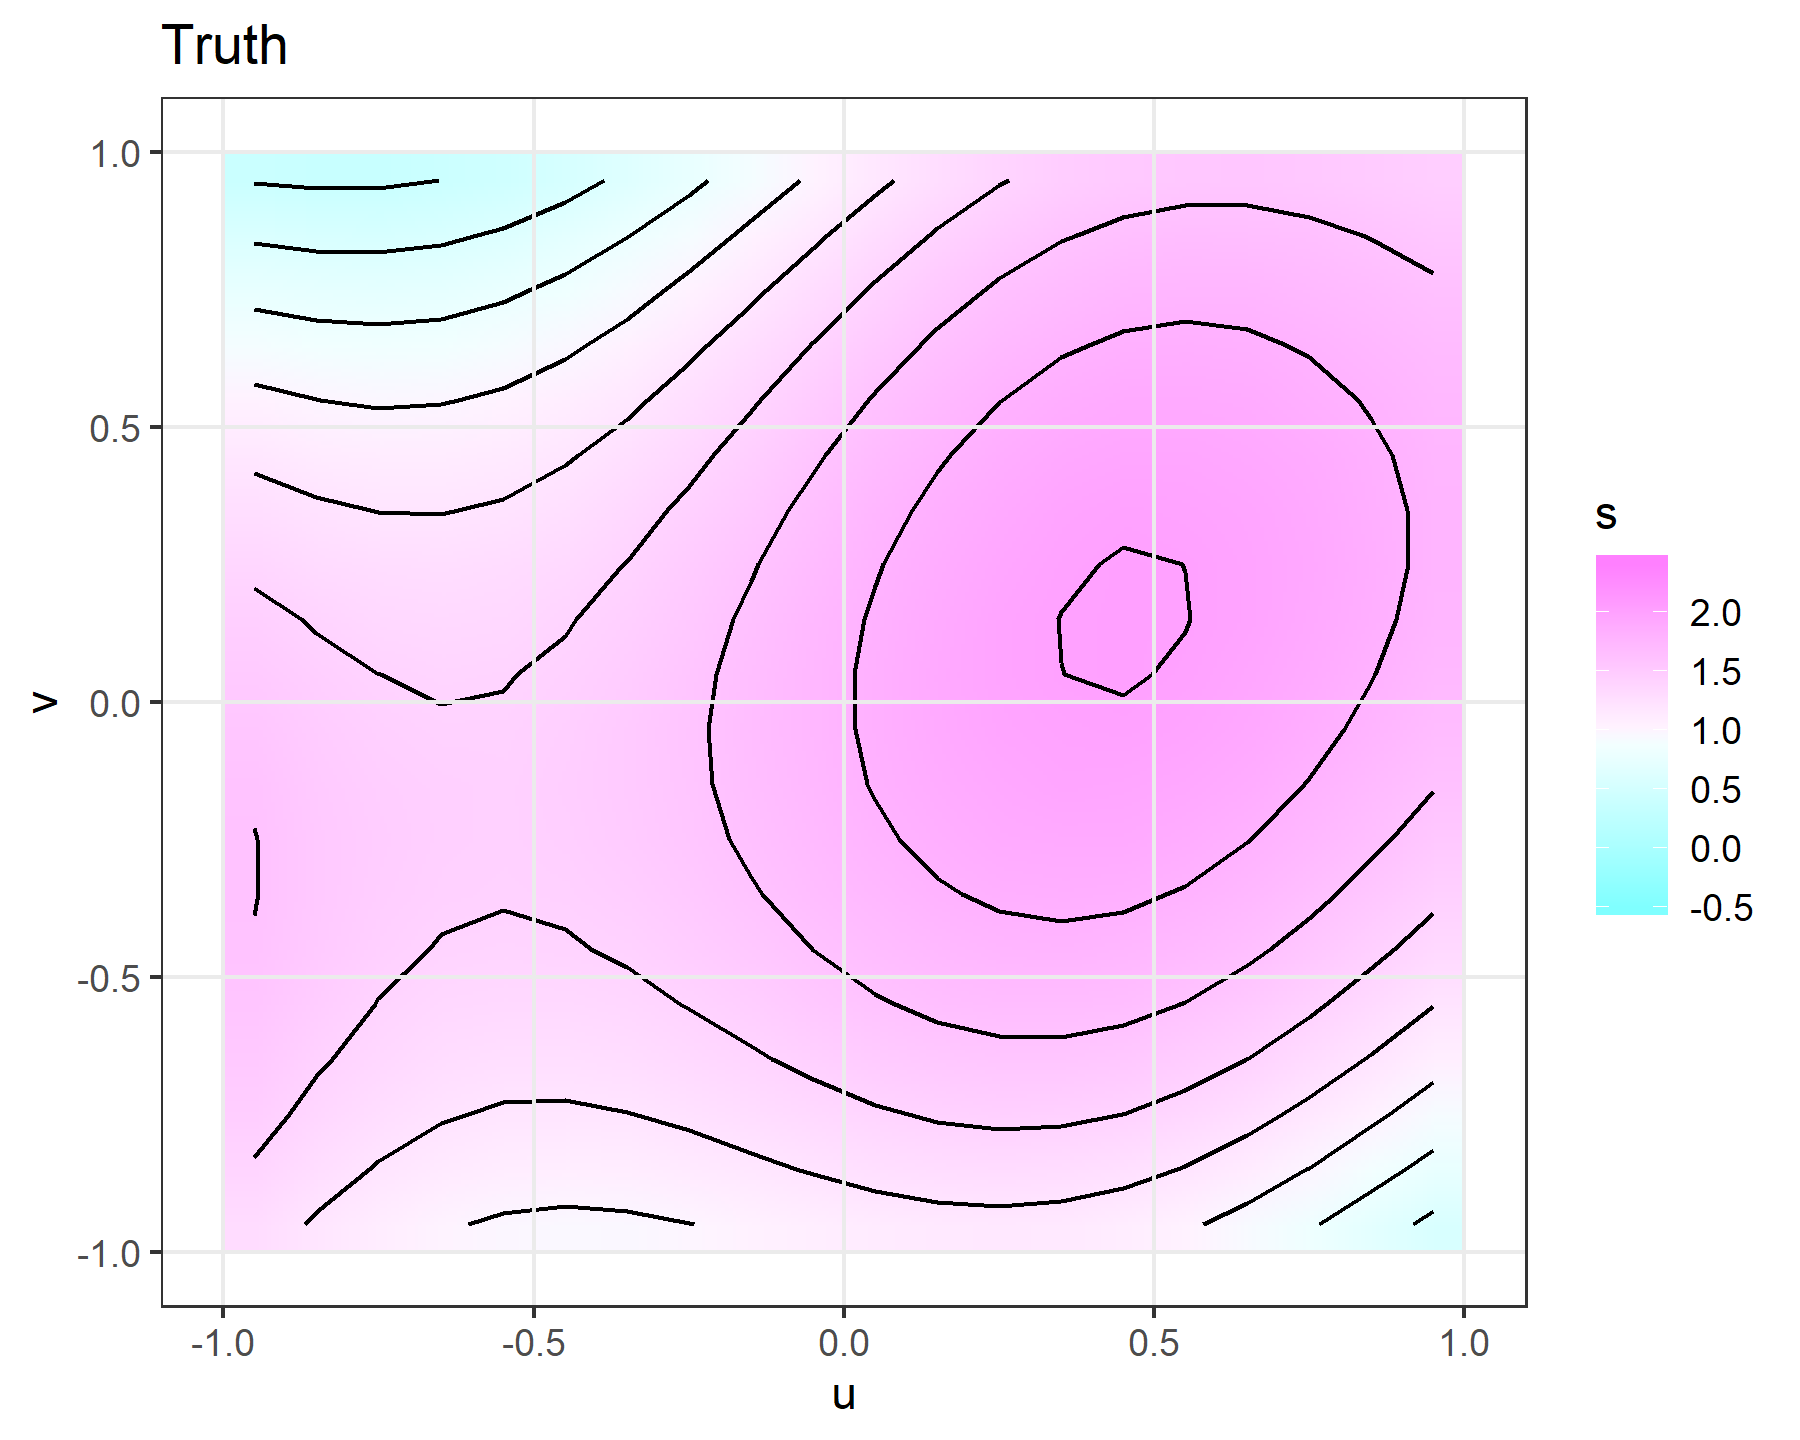
\includegraphics[width=0.4\linewidth]{Figures/Chap5/Paper3_true.png}
		\caption{Simulated spatial risk pattern.}
		\label{f:trueSpatial}
	\end{figure}
	
	\subsection{Spatial pattern recreation}
	In this section, we aimed to compare the performance of our proposed generalized additive mixed models in terms of spatial pattern recreation. Binary responses were then simulated via the model
	
	\begin{equation}\label{eq:simSP1}
	\mathbf{P}(y_{ij}=m) = p_{ij}^m(1-p_{ij})^{(1-m)},\ m=0,1
	\end{equation}
	where 
	\begin{equation}\label{eq:simSP2}
	\text{logit}(p_{ij}) = \beta_x x_{ij} + \beta_t t_{ij} + s_0(u_{ij},v_{ij}) + b_{0i} ,
	\end{equation}
	and $b_{0i} \stackrel{i.i.d.}{\sim} N(0,\tau_0^2)$. We repeated the simulation with $\tau_0=0,0.3,0.6,0.9$, respectively. 
	
	We sought to compare our proposed GAMM (given in (\ref{mod:gammsim})) with a naive GAM that assumes independent data (given in (\ref{mod:gamsim})):
	\begin{equation}\label{mod:gammsim}
	\text{logit}(p_{ij}) = \beta_0 +\beta_x x_{ij}+ \beta_t t_{ij} + lo(u_{ij},v_{ij}) + b_{0i} 
	\end{equation}
	\begin{equation}\label{mod:gamsim}
	\text{logit}(p_{ij}) = \beta_0 + \beta_x x_{ij}+ \beta_t t_{ij} + lo(u_{ij},v_{ij})
	\end{equation}
	
	We compared the estimated spatial risk patterns between the 2 models under varying random intercept conditions. Span sizes that minimize AIC \citep{akaike1998information} were chosen for classic GAM while our proposed OLMC method is used to choose span size for the GAMM. Note that if $\tau_0^2>0$, there will be individual-specific intercepts hence the model given in (\ref{mod:gamsim}) is a misspecified model due to its failure to account for the random effect. It follows that the likelihood of Model (\ref{mod:gamsim}) used in the AIC calculation would be incorrect hence the chosen span size tends not be the most appropriate, however a search across different span sizes did not return qualitatively different results from what is presented here. 
	
	The estimated spatial risk patterns are shown in Figure \ref{f:SpatialEsts3}. It is easily seen that that with correctly specified random effects, our proposed additive mixed models estimate the spatial patterns in a more precise fashion. In contrast, since the naive additive model fails to account for within-subject correlation, results for the model given in (\ref{mod:gamsim}) tend to under-smooth the patterns using a relatively small span sizes. This is due to the fact that the naive additive model treats correlated data as independent, resulting in an improper contribution of the correlated data to the total likelihood. 
	
	% f:SpatialEsts3 about here
	\begin{figure}[h]
		\centering
		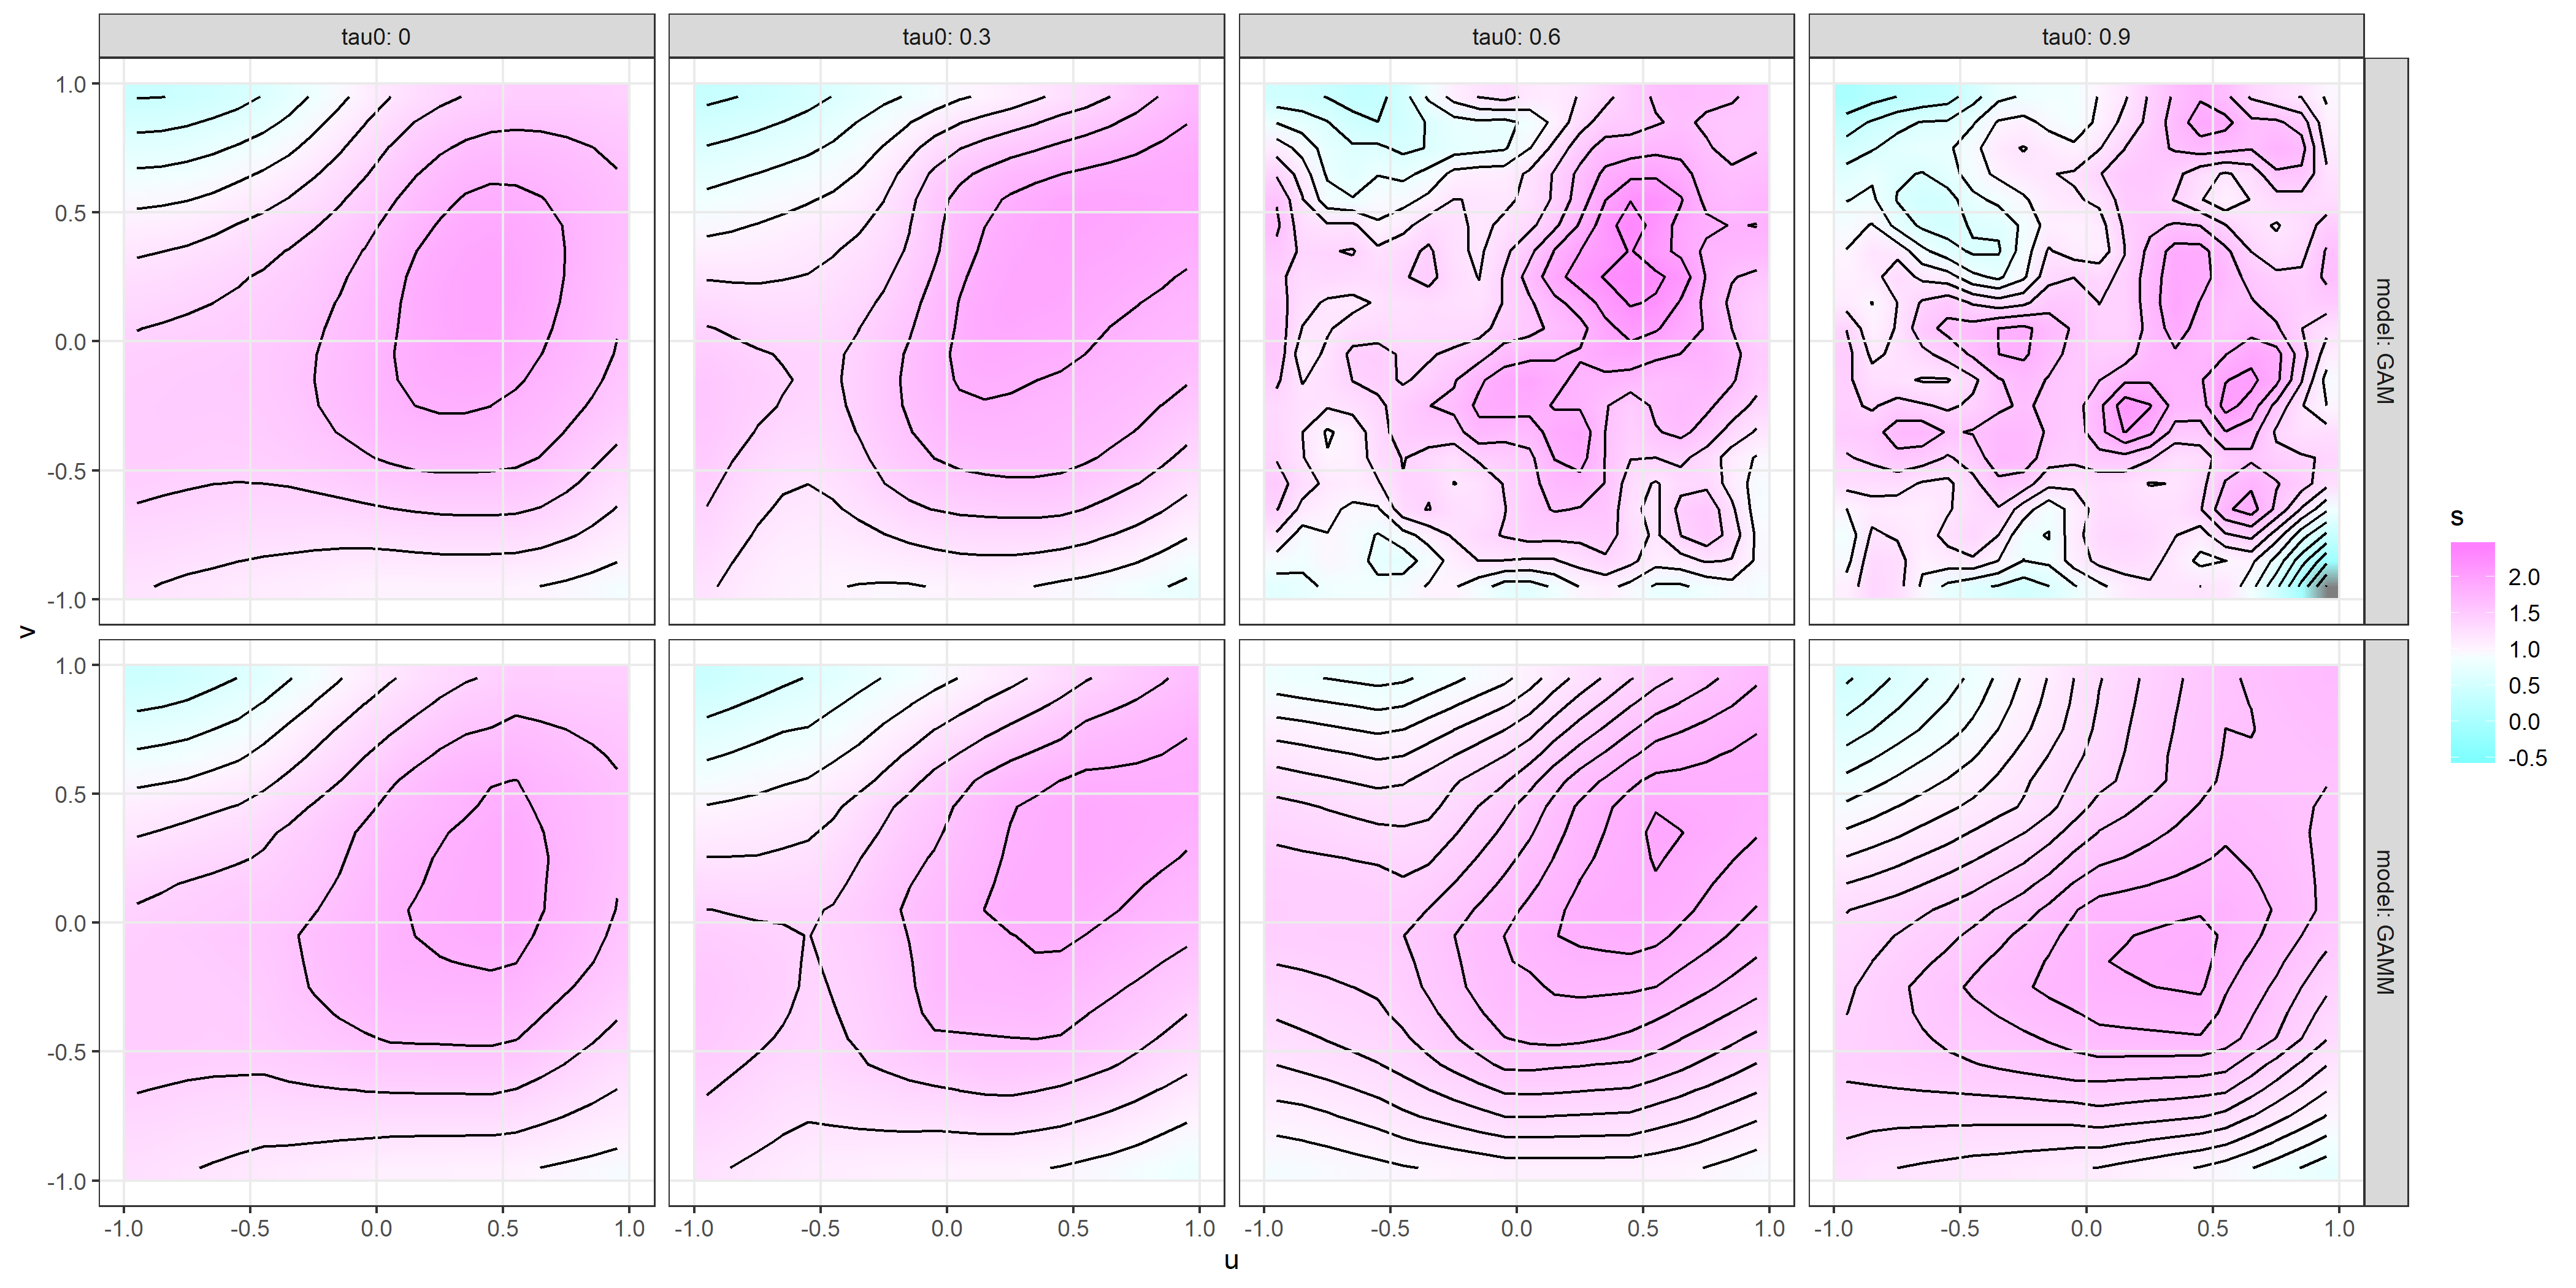
\includegraphics[width=1\linewidth]{Figures/Chap5/Comb_ests.png}
		\caption{Top: estimated patterns using GAMs given differing true correlation structures; Bottom : estimated patterns using GAMMs given differing true correlation structures.}
		\label{f:SpatialEsts3}
	\end{figure}
	
	\subsection{Quantification of uncertainty of estimated spatial effects}
	To access the performance of our proposed methods to quantify the uncertainty of estimated spatial effects discussed in \ref{s:fitting}, simulated data were created using (\ref{eq:simSP2}), where $b_{0i} \stackrel{i.i.d.}{\sim} N(0,\tau^2)$. 3 scenarios were designed with $\tau=0.2,\ 0.4,\ 0.6$, respectively. 300 repetitions were performed for each scenario. For each repetition, 95\% CIs are derived using our proposed method for every location on a uniformly designed $20\times 20$ grid on the map. Both sample mean and sample standard deviation of the coverage were reported in Table \ref{t:sim3coverage}. From the results, The uncertainty in spatial effects was well estimated and the 95\% confidence intervals managed to render the target coverage. 
	
	\begin{table}[h]
		\caption{Sample mean and sample standard deviation of the coverage proportion of 95\% confidence intervals of spatial effects. Coverage proportions are computed based on 300 repetitions while mean and standard deviation are calculated over 400 locations on map.
			\label{t:sim3coverage}}
		\centering
		\begin{tabular}{cccc}
			\hline
			$\tau_0$ & mean coverage & s.d. \\
			\hline
			0.2 &  0.939 & 0.039\\
			0.4 &  0.947 & 0.055\\
			0.6 &  0.979 & 0.030\\
			\hline
		\end{tabular}
	\end{table}
	
	\subsection{Parameter estimation}
	In this section, we investigated the performance of our proposed GAMMs in terms of point estimation of the parameters in both the fixed effects and the variance of random effects via a new set of simulation studies where responses were simulated using model 
	\begin{equation}\label{eq:simrand}
	\text{logit}(p_{ij}) = \beta_x x_{ij} + \beta_t t_{ij} + s_0(u_{ij},v_{ij}) + b_{0i} + b_{1i}t_{ij},
	\end{equation}
	with $b_{0i} \stackrel{i.i.d.}{\sim} N(0,\tau_{0}^2)$ and $b_{1i} \stackrel{i.i.d.}{\sim} N(0,\tau_{1}^2)$.
	
	On the simulated dataset, we sought to access the performance of our proposed GAMM given by 
	\begin{equation}\label{mod:ammsim2}
	y_{ij} = \beta_0 + \beta_x x_{ij} + \beta_t t_{ij} + lo(u_{ij},v_{ij}) + b_{0i} + b_{1i}t_{ij}.
	\end{equation}
	The estimated values of $\beta_x$, $\beta_t$, $\tau_{0}$ and $\tau_{1}$ were recorded. The corresponding results presented in Table \ref{t:parameterests} were based upon a total of 300 simulations. The sample mean and standard deviation of estimated model parameters, along with the mean estimated standard deviations, were reported. From the results, it could be seen that by correctly accounting for the correlation structure, our proposed GAMMs managed to both estimate parameters in fixed effects with less bias. On the other hand, GAMMs accounted for the individual-specific random effects and hence managed to estimate the variance of the random effects. 
	
	% t:parameterests about here
	% latex table generated in R 3.6.0 by xtable 1.8-4 package
	% Sat Jul 25 16:02:17 2020
	\begin{table}[h]
		\caption{Parameter estimation based on 300 repetitions
			\label{t:parameterests}}
		\centering
		\begin{tabular}{llrrlll}
			\hline
			model & parameter & truth & mean of estimates & relative bias & empirical s.d. & mean of $\hat{s.d.}$ \\     \hline
			GAM & $\beta_x$ & 0.20 & 0.17 & -17\% & 0.033 & 0.031 \\ 
			& $\beta_t$ & -0.10 & -0.09 & 12\% & 0.0034 & 0.0032 \\ 
			GAMM & $\beta_x$ & 0.20 & 0.19 & -5.5\% & 0.035 & 0.032 \\ 
			& $\beta_t$ & -0.10 & -0.10 & 4\% & 0.004 & 0.0041 \\ 
			& $\tau_0$ & 0.50 & 0.53 & 6.6\% & - & - \\ 
			& $\tau_1$ & 0.07 & 0.07 & -5.7\% & - & - \\ 
			\hline
		\end{tabular}
	\end{table}
	
	
	\section{Application to serum PFOA study}
	In this section, we apply our proposed GAMM to estimate the spatial risk pattern of high serum PFOA concentration with adjustment of relevant confounding covariates. Here we focus on a approximate square map defined within longitude $81^{\circ} 30'\  W$ - $81^{\circ} 50'\  W$ and latitude $39^{\circ} 07'\  N$ - $39^{\circ} 27'\  N$, which is approximately a $23\times 23$ square in miles around Lubeck, WV area. Within this area, 1070 records on 193 individuals are available where 140 of them have 6 measurements of serum PFOA concentration. Among the 193 residents, 99 are female and 94 are male. Age at baseline has mean 54.6 and standard deviation 14.9 with minimum 19 and maximum 92. We use 100 ng/mL as a threshold for ``high concentration" where serum PFOA concentration values that are greater than 100 ng/mL are considered high. 
	
	To estimate the spatial pattern of residents' high serum PFOA concentration risk with control of gender, age and a linear trend in time, we fitted an GAMM given by 
	
	\begin{equation}\label{mod:PFOA}
	g(p_{ij}) = \beta_0 + \beta_1 female_i + \beta_2 age_i + \beta_3 t_{ij} + lo(u_{ij}, v_{ij}) +  b_{0i}, 
	\end{equation}
	where $p_{ij}$ is the probability that individual $i$ has a high serum PFOA concentration at time $j$ and $b_{0i} \stackrel{i.i.d.}{\sim} N(0,\tau_0^2)$. 
	
	The fitted spatial pattern of log-odds, along with point-wise 95\% confidence intervals, is shown in Figure \ref{f:pfoaplotsGAMM}. From the results, it could be seen that potential high PFOA risk areas exist in western and north-eastern parts of the area. Further point-wise significance tests are performed at each location within a uniformly designed $20\times 20$ grid on the map of interest. Specifically, 95\% confidence interval of spatial effect at each location is compared with the mean estimated spatial effect over the 400 locations. A location is labeled as significant if the 95\% CI at the location does not cover the mean estimated effect. The results are plotted in Figure \ref{f:pfoasigs3}, from which significantly higher risks are observed at 129 locations while significantly lower risks are observed at 175 locations, indicating significant geospatial disparity in residents' serum PFOA concentration over the map. These results could potentially help epidemiologists on further space-confounded risk factor detection. 
	
	
	\begin{figure}[h]
		\begin{center}
			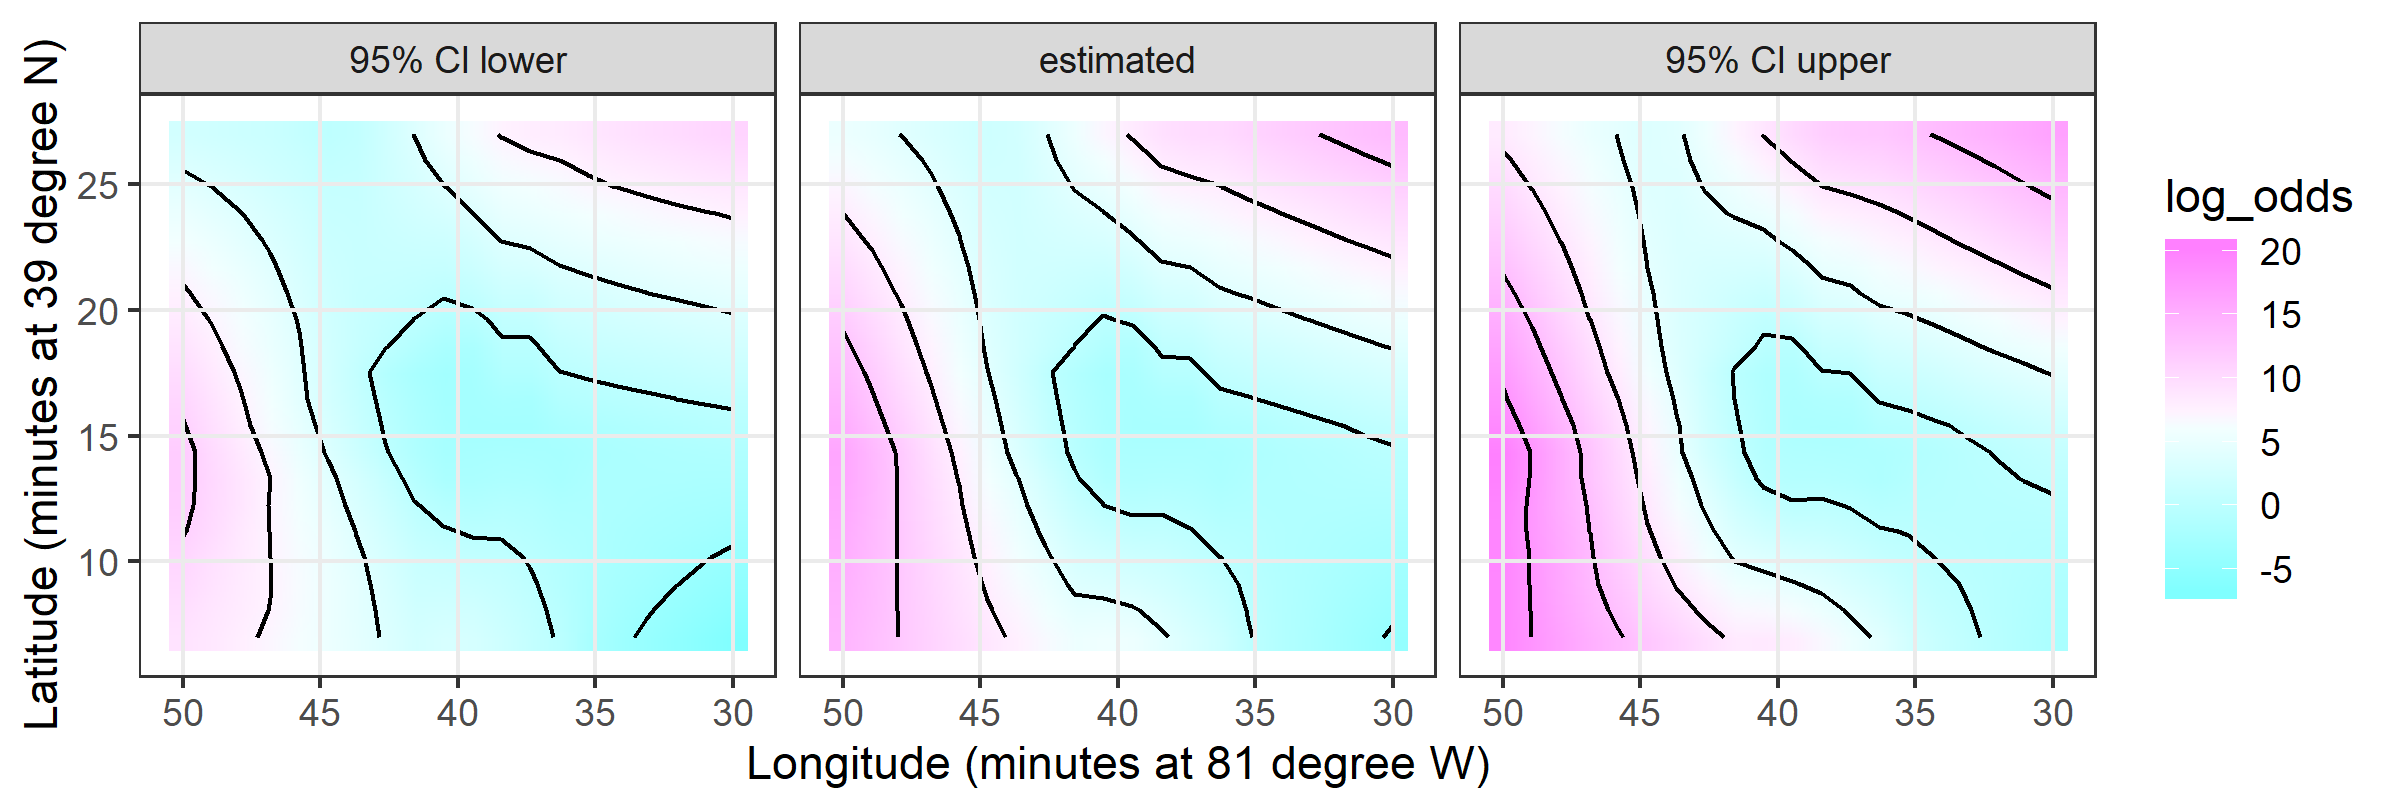
\includegraphics[width=\linewidth]{Figures/Chap5/Ests3.png}
		\end{center}
		\caption{Left: point-wise lower bounds of 95\% CIs ; Middle: estimated pattern of log odds ratio of high serum PFOA using Model (\ref{mod:PFOA}); Right: point-wise upper bounds of 95\% CIs.}
		\label{f:pfoaplotsGAMM}
	\end{figure}
	
	\begin{figure}[h]
		\begin{center}
			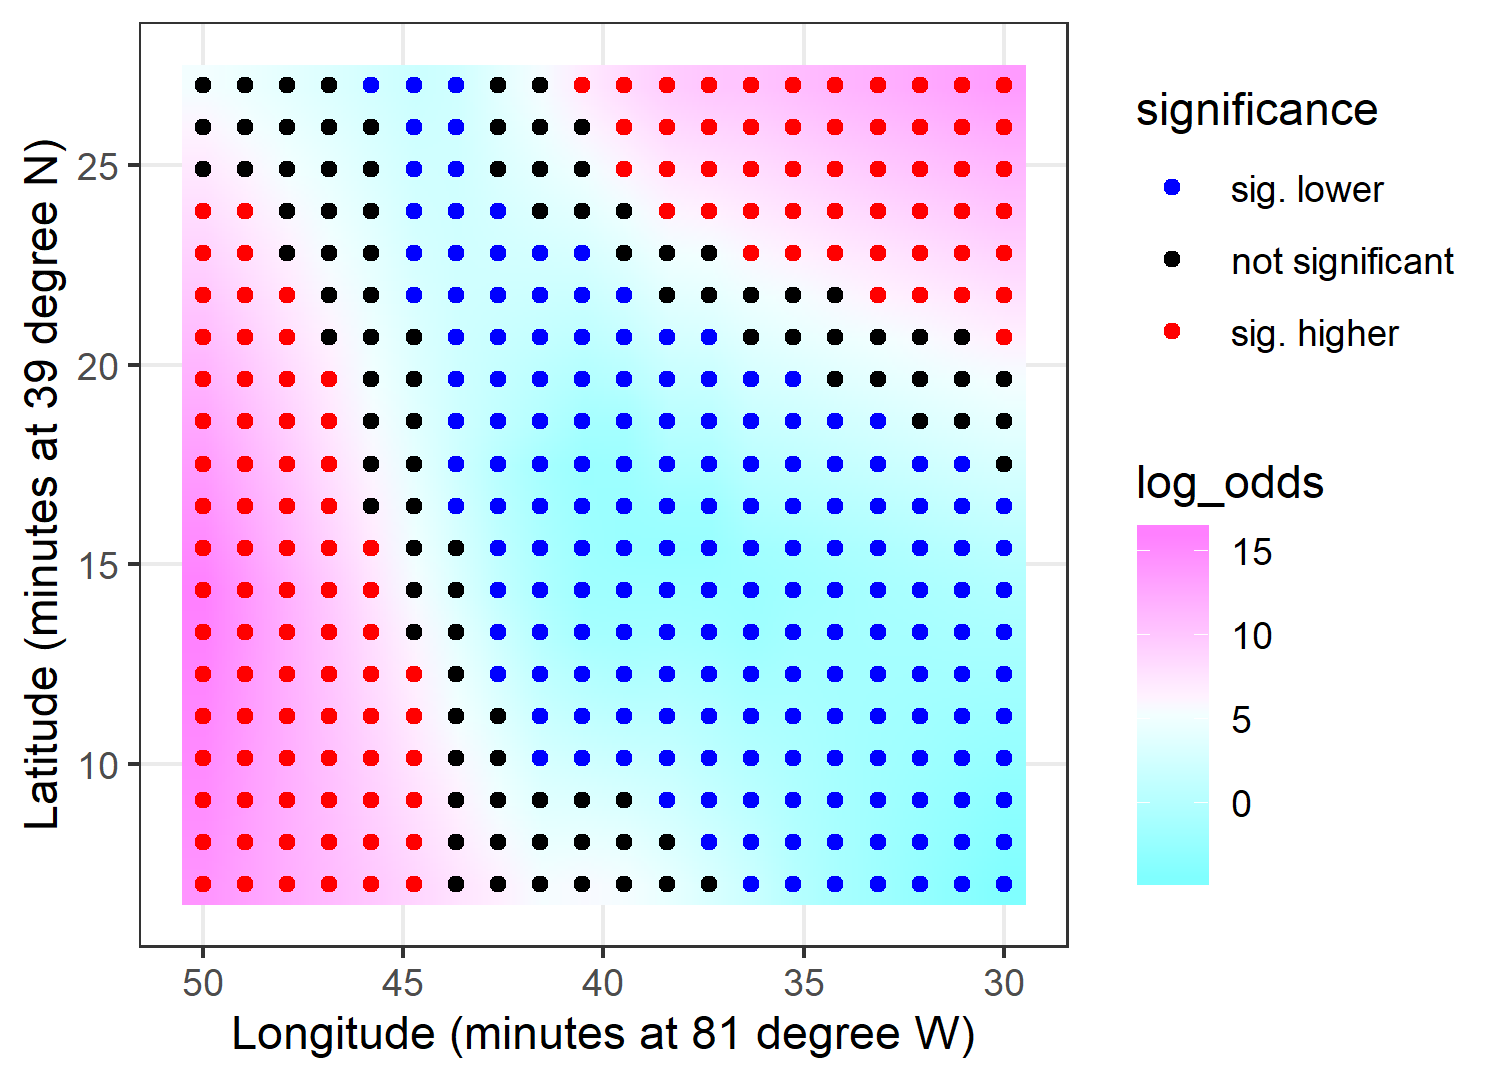
\includegraphics[width=0.5\linewidth]{Figures/Chap5/sig3.png}
		\end{center}
		\caption{Significance of the grid locations on the estimated spatial effects map.}
		\label{f:pfoasigs3}
	\end{figure}
	
	\section{Discussion}
	\label{s:discuss}
	We proposed a novel class of generalized additive mixed models that incorporate kernel smoothers. To achieve this, we combined PQL procedure and backfitting algorithm. To choose the proper amount of smoothing, we proposed an out-of-sample likelihood Monte Carlo method in order to avoid over-smoothing or under-smoothing. We showed that by adjusting for the correlation structure, our model better recreated the spatial risk pattern than a naively applied GAM. Empirical results also showed that our model managed to render estimation of parameters in both mean and variance components with less bias when the model was correctly specified. Our methods were further used in a recent study on residents' serum PFOA concentration in Lubeck, WV and spatial disparity in risk of high serum PFOA concentration was identified. 
	
	In this work, we focused on kernel smoothers, utilizing LOESS in particular in order to meet the demand of various spatial epidemiology studies. We mentioned but did not elaborate on the use of spline smoothers in the context, partially due to the fact that those models are relatively well investigated in existing literature such as \citet{wood2017generalized} and \citet{lin1999inference}. We did not cover Bayesian spatial estimation methods based on stochastic processes but we do recognize their popularity, as well.
	
	This work is a direct complement of the work of \citet{Tang2020Additive} by accommodating responses of exponential family. This work could also be viewed as the alternative to \citet{lin1999inference} when kernel smoothers are preferred over spline smoothers. This work was developed based on PQL procedure, which is one of the popular fitting procedure of a classic GLMM. One natural future direction is to develop a fitting procedure using marginal quasi-likelihood \citep{breslow1993approximate} for GAMM with kernel smoothers. 
	
	

%%% Local Variables: ***
%%% mode: latex ***
%%% TeX-master: "thesis.tex" ***
%%% End: ***

%\chapter{Discussion}

Using disease mapping problems in spatial epidemiology studies as motivation, this dissertation work extended GAM framework in order to accommodate studies that look at data over a certain period of time. In Chapter 3, we proposed time-stratified bivariate kernel smoothers and incorporated them into classic GAM framework. To test the significance of stratification, we adopted a permutation strategy, bringing in a class of PMSD tests. In Chapters 4 and 5 concentrated on disease mapping problems in longitudinal analysis. Chapter 4 filled the gap in literature and proposed a class of AMMs that model fixed effects, random effects and spatial effects simultaneously for Gaussian distributed responses. Chapter 5 further released the restriction on distribution of response and constructed GAMMs with kernel smoothers. Chapters 4 and 5 combined could be viewed as a counterpart and complementation of \citet{lin1999inference}, offering an option for researchers who aim to use LOESS or other kernel smoothers in mixed models. 

We would also like to mention that, other than a frequentist GAM framework, Bayesian disease mapping techniques, which commonly utilize Gaussian process or other types of stochastic processes for spatial effects estimation, are popular in spatial analysis as well. Bayesian methods could be more flexible if hierarchical structure is well adopted. Bayesian methods also enjoy direct inference on random effects and unified framework in inference on the whole model without approximate derivation or backfitting procedures. Nevertheless, Bayesian methods require good experience in model setup, prior distribution selection and MCMC controlling, all of which are hardly trivial to non-statisticians or even statisticians who have little expertise in geospatial analysis. In addition, when data set groups large, GAM and its extensions are generally considered more scalable. 

Along the avenue of this study, some future directions are attractive. The GAMMs in Chapter 5 used PQL procedure hence to complete the whole framework, similar work could be done for MQL procedure. Also, we noticed that in mixed models with exponential family responses, Bernoulli response in particular, the uncertainty in marginal trend parameter could not be correctly accounted for. We believe generalized estimation equations are worth investigating to solve this issue. On the other hand, this work did not consider the modeling of censored data. Therefore incorporation of the proposed methods into survival analysis framework, cox proportional hazard model in particular, should be further investigated.

%%% Local Variables: ***
%%% mode: latex ***
%%% TeX-master: "thesis.tex" ***
%%% End: ***

% ... and so on

% These commands fix an odd problem in which the bibliography line
% of the Table of Contents shows the wrong page number.
\clearpage
\phantomsection

% "References should be formatted in style most common in discipline",
% abbrv is only a suggestion.
%\bibliographystyle{abbrv}
\bibliographystyle{plainnat}
\bibliography{2randCiting.bib}

% The Thesis Manual says not to include appendix figures and tables in
% the List of Figures and Tables, respectively, so these commands from
% the caption package turn it off from this point onwards. If needed,
% it can be re-enabled later (using list=yes argument).
\captionsetup[figure]{list=no}
\captionsetup[table]{list=no}

% If you have an appendix, it should come after the references.
%\begin{appendices}
%\include{appendix}
%\end{appendices}

\end{document}
